%!TEX root = ../report.tex
\documentclass[report.tex]{subfiles}
\begin{document}
    \chapter{Methodology}
        % Dont know where to put DATASET related content
    % One entire section could be my comparative study on multimodal dataset
    \section{Available Datasets}

    % \begin{itemize}
    %     \item The majority of deep multimodal perception approaches rely on supervised learning, and therefore necessitate multimodal datasets with labeled ground truth for training deep neural networks. While several multimodal datasets are available, many of these datasets are collected under clear weather conditions or do not include all sensors, such as cameras, LiDAR, and radar. Unfortunately, the availability of multimodal datasets collected under adverse weather conditions with all three sensors are limited. Table 1 summarizes some of the available multimodal datasets for evaluating the performance of deep multimodal perception techniques in adverse weather conditions. Of these datasets, only the recently released K-Radar \cite{Paek2022Jun} incorporates a high-resolution 4D-radar sensor. In the table, C-R-L-N-F denotes the Camera, Radar, LiDAR, Near-infrared, and Far-infrared sensors, respectively.
    %         \begin{table}[h]
    %             \centering
    %             \caption{List multimodal datasets with adverse weather conditions}
    %             \label{tab:my-table}
    %             \begin{tabular}{|l|l|l|l|}
    %                 \hline
    %                 \textbf{Name}       & \textbf{Sensors} & \textbf{Reference}               & \textbf{Year} \\ \hline
    %                 DENSE               & CRLNF            & \cite{bijelic2020seeing}    & 2020          \\ \hline
    %                 EU Long-term        & CRL              & \cite{yan2020eu}            & 2020          \\ \hline
    %                 nuScenes            & CRL              & \cite{caesar2020nuscenes}   & 2020          \\ \hline
    %                 The Oxford RobotCar & CRL              & \cite{barnes2020oxford}     & 2020          \\ \hline
    %                 RADIATE             & CRL              & \cite{sheeny2021radiate}    & 2021          \\ \hline
    %                 K-Radar             & CRL              & \cite{Paek2022Jun}          & 2022          \\ \hline
    %                 aiMotive            & CRL              & \cite{matuszka2022aimotive} & 2022          \\ \hline
    %                 Boreas              & CRL              & \cite{burnett2022boreas}    & 2022          \\ \hline
    %                 WADS                & CRLNF            & \cite{kurup2022winter}      & 2023          \\ \hline
    %             \end{tabular}
    %         \end{table}

    %         \begin{figure}[h]
    %             \centering
    %             \includegraphics[width=1.0\textwidth]{images/all_sensors_in_adverse_weather.png}
    %             \caption{\centering Samples of K-Radar datasets for various weather conditions \cite{Paek2022Jun}}
    %             \label{fig:all_sensors_in_adverse_weather}
    %         \end{figure}
    %     \end{itemize}


    The majority of deep multimodal perception approaches rely on supervised learning, which necessitates the use of high-quality, large-scale multimodal datasets with labeled ground truth for training deep neural networks. Several multimodal datasets, such as KITTI \cite{geiger2012we}, ApolloScape \cite{huang2019apolloscape}, and Waymo \cite{sun2020scalability}, are prevalent in the domain of LiDAR-camera fusion. However, a significant number of these datasets are collected under clear weather conditions or lack a comprehensive array of sensors, including cameras, LiDAR, and Radar. A notable limitation is the scarcity of multimodal datasets that are collected under adverse weather conditions and incorporate at least all three of these essential sensors. Table \ref{datasets} summarizes some of the available multimodal datasets\footnote{For all the datasets, formal registration form is required to fill to access the dataset} for evaluating the performance of deep multimodal perception techniques in adverse weather conditions. The dataset are sorted in ascending order with respect to year.

    \begin{table}[!ht]
        \centering
        \caption{Multimodal adverse weather conditions datasets. Sensors†: C-R-L-N-F denote Camera, Radar, LiDAR, Near-infrared, and Far-infrared sensors, respectively. Weather conditions‡: F-SN-R-O-SL-N denote Fog, Snow, Rain, Overcast, Sleet, and Night conditions, respectively. Note that highlighted datasets are used for the project.}
        \begin{tabular}{|l|l|l|l|l|l|l|}
        \hline
            \textbf{Name} & \textbf{Sensors†} & \textbf{Weather Cond.‡} & \textbf{Size (GB)} & \textbf{Year} & \textbf{Citation Cnt.} & \textbf{Ref.} \\ \hline
            \textbf{DENSE} & \textbf{CRLNF} & \textbf{F, SN, R, O, N} & \textbf{582} & \textbf{2020} & \textbf{269} & \textbf{\cite{bijelic2020seeing}} \\ \hline
            \textbf{nuScenes} & \textbf{CRL} & \textbf{R, N} & \textbf{400} & \textbf{2020} & \textbf{3459} & \textbf{\cite{caesar2020nuscenes}} \\ \hline
            Oxford RobotCar & CRL & R, SN, F & 4700 & 2020 & 317 & \cite{barnes2020oxford} \\ \hline
            EU Long-term & CRL & SN, R, O, N & NA & 2020 & 72 & \cite{yan2020eu} \\ \hline
            RADIATE & CRL & F, SN, R, O, SL, N & NA & 2021 & 132 & \cite{sheeny2021radiate} \\ \hline
            K-Radar & CRL & F, R, SN & 13000 & 2022 & 15 & \cite{Paek2022Jun} \\ \hline
            Boreas & CRL & SN, R, O, N & 4400 & 2022 & 38 & \cite{burnett2022boreas} \\ \hline
            aiMotive & CRL & R, O, N & 85 & 2023 & 3 & \cite{matuszka2022aimotive} \\ \hline
        \end{tabular}
        \label{datasets}
    \end{table}


    % The datasets for the project are selected based on the following criteria:
    % - Available Sensors, at least it should have camera, radar, and lidar
    % - Adverse weather conditions,
    % - Dataset documentation and accessibility,
    % - Usage by publicly available methods (so that comparison is possible)
    % - Perception Task, eg. Object Detection
    % - Radar datatype, the data should be available in point cloud format
    % - Time-synchronized and calibrated data

    % After considering above criteria, the following datasets are selected (also highlighted in the table): 
    % - DENSE
    % - nuScenes

    The selection of appropriate datasets is crucial. The criteria for selecting datasets cover several key areas, focusing on the availability of diverse sensors, specifically cameras, radar, and lidar, which are crucial for robust object detection in challenging environments. Additionally, the datasets must represent adverse weather conditions effectively, as this is a critical aspect of the research. Furthermore, the accessibility and thorough documentation of the datasets are considered, ensuring that the data can be easily understood and utilized in the research process. Another vital criterion is the dataset's popularity in existing research, as this allows for comparative analysis with publicly available methods, thereby validating the research findings. Moreover, the specific perception task, in this case, object detection, and the type of radar data, particularly in point cloud format, are essential considerations. The requirement for time-synchronized and calibrated data is also emphasized to ensure accuracy and reliability in sensor fusion and object detection algorithms.

    After a comprehensive evaluation of these criteria, two datasets have been chosen for this research: DENSE and nuScenes. The DENSE dataset is particularly suited for this study as it includes data from various sensors under adverse weather conditions, which is crucial for testing the efficacy of multimodal sensor fusion in challenging environments. The nuScenes dataset, on the other hand, is widely used in the field, providing a rich source of data with camera, radar, and lidar sensors. Its extensive use in the community allows for a meaningful comparison with existing methods. Both datasets provide time-synchronized and calibrated data, which is essential for the accuracy of object detection algorithms in adverse weather conditions. The selection of these datasets aligns perfectly with the research objectives, offering a comprehensive platform for exploring and advancing the capabilities of data-driven multimodal sensor fusion in object detection under challenging weather scenarios.

    \subsection{DENSE dataset}

    % The Dense dataset \cite{bijelic2020seeing} focused on evaluating multi-modal fusion algorithms under adverse weather. In addition to LiDAR and a stereo camera, it is also equipped with several all-weather sensors, including one frontal long-range radar, one gated camera working on the NIR band, one FIR camera, and one weather station sensor. The data are captured in various natural weather conditions, including rain, snow, light fog, and heavy fog, as well as in a controlled lab environment in a fog chamber. However, the dataset only provides sparse radar targets with limited FoV and low resolution. 
    % - The dataset is recorded in urban city, suburban, highway, and tunnel areas. 
    % - It coveres several weather conditions like light fog, dense fog, rain, snow, and night. The dataset is used by several multimodal sensor fusion publications for object detection. 
    % - Table \ref{tab:dataset_comparison} higlihts the sensor setup and dataset statistics for each dataset. 
    % - Geographical coverage of the data collection campaign covering two months and 10,000 km in Germany, Sweden, Denmark, and Finland. 
    % - DENSE dataset provides Radar targets in point cloud format.
    % - As Radar data points are inherently noisy, so the both datasets have already been preprocessed to remove the false points.
    % - Radar data directly provide 3D information consisting of range, azimuth, and velocity. As an additional note, new generation Radar sensors provide 4D data with range, azimuth, velocity, and elevation.
    % - It provides 2D annotations in COCO style format, where bbox format is x, y, width, height.
    The DENSE dataset, as detailed in Bijelic et al. (2020) \cite{bijelic2020seeing}, is a critical asset for evaluating multi-modal fusion algorithms in adverse weather conditions. Its standout feature is the extensive sensor array, including LiDAR, a stereo camera, a frontal long-range radar, a gated camera operating in the NIR band, a FIR camera, and a weather station sensor, as illustrated in Figure \ref{fig:dense_test_vehicle_setup}. These sensors allow for detailed data capture under various adverse weather conditions, such as rain, snow, light fog, and dense fog. Notably, the DENSE dataset uniquely offers a split for light and dense fog conditions, essential for assessing the detection performance of Lidar and Radar in varying visibility scenarios. The range of these conditions and their distribution are visually depicted in Figure \ref{fig:dense_distribution_of_weather_conditions}. Additionally, the dataset includes data from a controlled lab environment within a fog chamber, offering a distinct view of sensor performance under simulated conditions. However, it's important to note that for the purposes of this project, only real-world data from the DENSE dataset is utilized. A few random samples from the dataset are shown in Figure \ref{fig:dense_samples}. Note that LiDAR and Radar points are projected onto the camera image for visualization purposes.

    The dataset covers a broad spectrum of environments, encompassing urban cities, suburban areas, highways, and tunnels. Its geographical scope is extensive, with data collection spanning over two months and covering 10,000 km across Germany, Sweden, Denmark, and Finland. This diverse environmental range enhances the dataset's applicability in various real-world scenarios.

    Technically, the DENSE dataset offers radar targets in a point cloud format, aligning well with the Lidar data. Given the inherent noise in radar data, preprocessing has been performed to eliminate false points, thereby bolstering the dataset's accuracy and reliability. The radar data includes 3D information - range, azimuth, and velocity. Moreover, it's noteworthy that the latest generation of radar sensors in the dataset provides 4D data, adding elevation to the existing dimensions. There are total 3 classes available in the dataset, including car, pedestrian, and cyclist. Object annotations in the DENSE dataset are provided in 2D as well in 3D format, and follow the COCO style format \cite{lin2014microsoft}, with bounding box (bbox) parameters specified as x, y, width, and height. The annotation processed is well described in the supplementary material from the paper \cite{heide2023adverseweatherfusion}. This meticulous approach to data collection, processing, and annotation positions the DENSE dataset as a powerful and adaptable tool for research in adverse weather conditions, especially in the domain of data-driven multimodal sensor fusion.

        % \begin{figure}[h]
        %         \centering
        %         \includegraphics[width=0.5\textwidth]{images/datasets/dense/test_vehicle_setup.png}
        %         \caption{Test Vehicle Setup \cite{bijelic2020seeing}}
        %         \label{fig:dense_test_vehicle_setup}
        % \end{figure}

        % \begin{figure}[h]
        %         \centering
        %         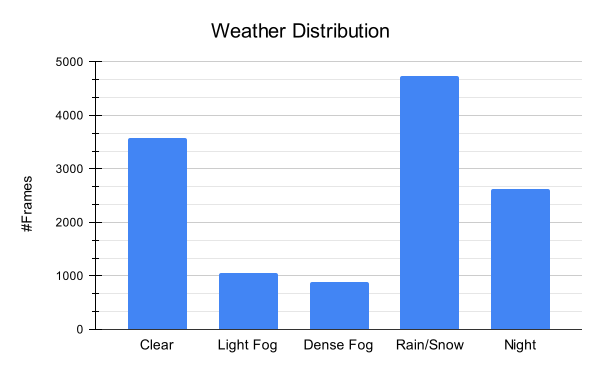
\includegraphics[width=0.5\textwidth]{images/datasets/dense/distribution_of_weather_conditions.pdf}
        %         \caption{Distribution of Weather Conditions \cite{bijelic2020seeing}}
        %         \label{fig:dense_distribution_of_weather_conditions}
        % \end{figure}

        \begin{figure}[h]
            \centering
            \begin{minipage}{0.45\textwidth}
                \centering
                \includegraphics[width=\textwidth]{images/datasets/dense/test_vehicle_setup.png}
                \caption{Test vehicle setup (Image source \cite{bijelic2020seeing})}
                \label{fig:dense_test_vehicle_setup}
            \end{minipage}
            \hfill
            \begin{minipage}{0.45\textwidth}
                \centering
                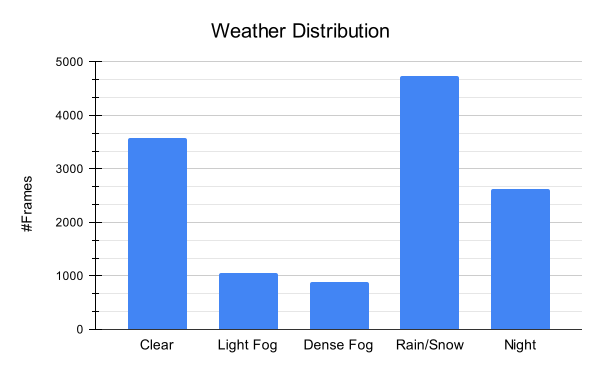
\includegraphics[width=\textwidth]{images/datasets/dense/distribution_of_weather_conditions.pdf}
                \caption{Distribution of weather conditions \cite{bijelic2020seeing}}
                \label{fig:dense_distribution_of_weather_conditions}
            \end{minipage}
        \end{figure}
        

        % TODO: add Classwise distribution
        % \begin{figure}[h]
        %     \centering
        %     \includegraphics[width=0.9\textwidth]{images/datasets/dense/classwise_distribution.png}
        %     \caption{Classwise Distribution \cite{bijelic2020seeing}}
        %     \label{fig:dense_classwise_distribution}
        % \end{figure}

        \begin{figure}[ht!]
            \centering
            % Row 1
            \includegraphics[width=0.3\textwidth]{images/datasets/dense/samples/day/2018-02-05_12-07-39_00300.png}\hfill
            \includegraphics[width=0.3\textwidth]{images/datasets/dense/samples/day/clean_lidar.png}\hfill
            \includegraphics[width=0.3\textwidth]{images/datasets/dense/samples/day/clean_radar_annotated.png}
          
            % Row 2
            \includegraphics[width=0.3\textwidth]{images/datasets/dense/samples/light_fog/2018-10-08_08-10-40_02160.png}\hfill
            \includegraphics[width=0.3\textwidth]{images/datasets/dense/samples/light_fog/light_fog_lidar.png}\hfill
            \includegraphics[width=0.3\textwidth]{images/datasets/dense/samples/light_fog/light_fog_radar_ann.png}
          
            % % Row 3
            \includegraphics[width=0.3\textwidth]{images/datasets/dense/samples/dense_fog/2018-10-29_15-02-37_00580.png}\hfill
            \includegraphics[width=0.3\textwidth]{images/datasets/dense/samples/dense_fog/dense_lidar.png}\hfill
            \includegraphics[width=0.3\textwidth]{images/datasets/dense/samples/dense_fog/dense_radar_ann.png}
          
            % % Row 4
            \includegraphics[width=0.3\textwidth]{images/datasets/dense/samples/snow/2018-02-07_11-56-57_00520.png}\hfill
            \includegraphics[width=0.3\textwidth]{images/datasets/dense/samples/snow/snow_lidar.png}\hfill
            \includegraphics[width=0.3\textwidth]{images/datasets/dense/samples/snow/snow_radar_ann.png}
          
            % % Row 5
            \includegraphics[width=0.3\textwidth]{images/datasets/dense/samples/night/2018-02-09_18-50-50_00300.png}\hfill
            \includegraphics[width=0.3\textwidth]{images/datasets/dense/samples/night/night_lidar.png}\hfill
            \includegraphics[width=0.3\textwidth]{images/datasets/dense/samples/night/night_radar_ann.png}
          
            \caption{Random samples from the DENSE dataset, where 1st column is Camera with ground truth, 2nd is LiDAR, 3rd is Radar (1st Row: Day, 2nd Row: Light Fog, 3rd Row: Dense Fog, 4th Row: Snow, 5th Row: Night). Note: Radar sparse points are highlighted with a red ellipse. Best viewed in zoomed-in view.}
            \label{fig:dense_samples}
          \end{figure}
          


    \subsection{nuScenes dataset}

    % NuScenes \cite{caesar2020nuscenes} is the most popular dataset for its large-scale and diverse scenarios. The capturing vehicle is equipped with a 32-beam LiDAR, 6 cameras, 5 long-range multi-mode radars, and a GPS/IMU system. It provides 3D annotations of 23 classes of road users in 1000 scenes, with a total of 1.3 million frames. 
    % - Although, the Radar used in nuScenes has a sparse data, but it is good dataset to start with and also well documented. 
    % - The dataset is recorded in urban city, suburban, and highway areas.
    % - It coveres less adverse weather conditions compared to DENSE dataset, like rain and night.
    % - Table \ref{tab:dataset_comparison} higlihts the sensor setup and dataset statistics in comparison to DENSE.
    % - Geographical coverage of the data collection campaign covering 242 km in Boston and Singapore.
    % - It provides Radar targets in point cloud format same as DENSE dataset.
    % - Note that nuscenes dataset doesn't provide 2D annotations so the individual methods create their own 2D annotations based on the 3D annotations.
    % - After creating 2D annotations, the dataset is converted to COCO style format, where bbox format is x, y, width, height.

    In addition to the DENSE dataset, this project also uses the nuScenes dataset \cite{caesar2020nuscenes} as a benchmark. The nuScenes dataset stands out for its large-scale and diverse scenarios. The data collection vehicle for nuScenes, as depicted in Figure \ref{fig:nuscenes_test_vehicle_setup}, is equipped with a comprehensive set of sensors, including a 32-beam LiDAR, six cameras, five long-range multi-mode radars, and a GPS/IMU system. This dataset provides 3D annotations for 23 classes of road users across 1,000 scenes, accumulating to a total of 1.3 million frames. Although the radar data in nuScenes is sparse, its extensive documentation makes it a good starting point for research in object detection. A few random samples from the dataset are shown in Figure \ref{fig:nuscenes_samples}.

    The nuScenes dataset focuses on urban, suburban, and highway areas, but it covers fewer adverse weather conditions compared to the DENSE dataset, primarily rain and night scenarios, as shown in Figure \ref{fig:nuscenes_distribution_of_weather_conditions}. Like DENSE, nuScenes also provides radar data in point cloud format. There are total 23 classes but it can be categorize into 10 super classes, including car, truck, trailer, bus, construction vehicle, bicycle, motorcycle, pedestrian, traffic cone, and barrier. However, a notable distinction is that nuScenes does not provide 2D annotations. Researchers using this dataset typically generate their own 2D annotations based on the 3D annotations provided. Once these 2D annotations are created, the data is converted into the COCO style format \cite{lin2014microsoft}, similar to DENSE, where the bbox format includes x, y, width, and height dimensions.


        % \begin{figure}[h]
        %     \centering
        %     \includegraphics[width=0.9\textwidth]{images/datasets/nuscenes/test_vehicle_setup.png}
        %     \caption{Test Vehicle Setup \cite{bijelic2020seeing}}
        %     \label{fig:nuscenes_test_vehicle_setup}
        % \end{figure}

        % \begin{figure}[h]
        %     \centering
        %     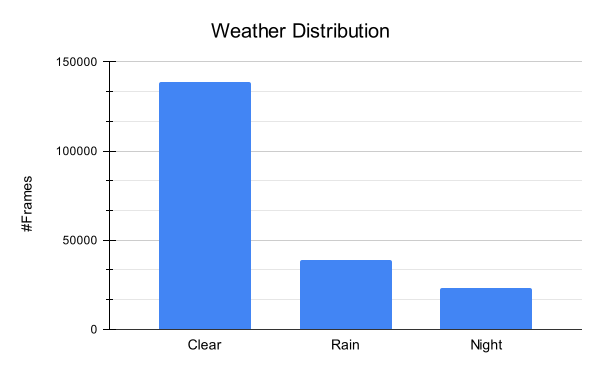
\includegraphics[width=0.9\textwidth]{images/datasets/nuscenes/distribution_of_weather_conditions.pdf}
        %     \caption{Distribution of Weather Conditions \cite{bijelic2020seeing}}
        %     \label{fig:nuscenes_distribution_of_weather_conditions}
        % \end{figure}

        \begin{figure}[h]
            \centering
            \begin{minipage}{0.48\textwidth}
                \centering
                \includegraphics[width=\textwidth]{images/datasets/nuscenes/test_vehicle_setup.png}
                \caption{Test vehicle setup (Image source \cite{caesar2020nuscenes})}
                \label{fig:nuscenes_test_vehicle_setup}
            \end{minipage}
            \hfill
            \begin{minipage}{0.48\textwidth}
                \centering
                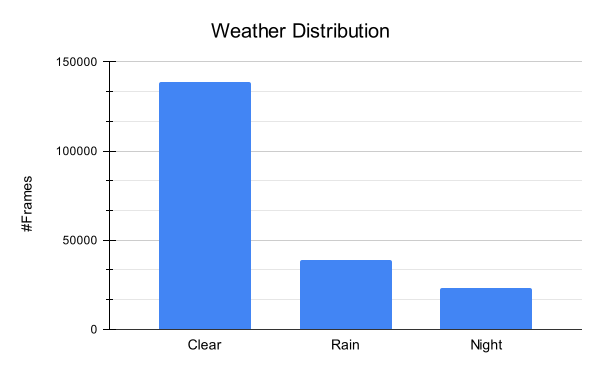
\includegraphics[width=\textwidth]{images/datasets/nuscenes/distribution_of_weather_conditions.pdf}
                \caption{Distribution of weather conditions \cite{caesar2020nuscenes}}
                \label{fig:nuscenes_distribution_of_weather_conditions}
            \end{minipage}
        \end{figure}
        

        % TODO: add Classwise distribution
        % \begin{figure}[h]
        %     \centering
        %     \includegraphics[width=0.9\textwidth]{images/datasets/nuscenes/classwise_distribution.png}
        %     \caption{Classwise Distribution \cite{bijelic2020seeing}}
        %     \label{fig:nuscenes_classwise_distribution}
        % \end{figure}

        % \begin{figure}[ht!]
        %     \centering
        %     % Row 1
        %     \includegraphics[width=0.3\textwidth]{images/datasets/nuscenes/samples/day_cam.png}
        %     \includegraphics[width=0.3\textwidth]{images/datasets/nuscenes/samples/night_cam.png}
          
        %     % Row 2
        %     \includegraphics[width=0.3\textwidth]{images/datasets/nuscenes/samples/rain_cam.png}
          
        %     \caption{A random samples from the nuScenes dataset Note: best viewed in color.}
        %     \label{fig:dense_samples}
        %   \end{figure}

          \begin{figure}[ht]
            \centering
            % First Image
            \begin{subfigure}{0.3\textwidth}
                \centering
                \includegraphics[width=\linewidth]{images/datasets/nuscenes/samples/day_cam.png}
                \caption{Day time}
                \label{fig:day_cam}
            \end{subfigure}
            \hfill
            % Second Image
            \begin{subfigure}{0.3\textwidth}
                \centering
                \includegraphics[width=\linewidth]{images/datasets/nuscenes/samples/night_cam.png}
                \caption{Night time}
                \label{fig:night_cam}
            \end{subfigure}
            \hfill
            % Third Image
            \begin{subfigure}{0.3\textwidth}
                \centering
                \includegraphics[width=\linewidth]{images/datasets/nuscenes/samples/rain_cam.png}
                \caption{Rain}
                \label{fig:rain_cam}
            \end{subfigure}
        
            \caption{Random samples from the nuScenes dataset}
            \label{fig:nuscenes_samples}
        \end{figure}
        

        Table \ref{tab:dataset_comparison} highlights the overall comparison of the sensor setup and dataset statistics for datasets used in this project.

        \begin{table}[h!]
            \centering
            \caption{Comparison of datasets features (Table adapted from \cite{bijelic2020seeing})}
            \begin{tabular}{|l|c|c|}
              \hline
              \textbf{Dataset} & \textbf{NuScenes \cite{caesar2020nuscenes}} & \textbf{DENSE \cite{bijelic2020seeing}} \\
              \hline
              RGB Cameras & 6 & 2 \\
              RGB Resolution & 1600x900 & 1920x1024 \\
              Lidar Sensors & 1 & 2 \\
              Lidar Resolution & 32 & 64 \\
              Radar Sensor & 4 & 1 \\
              Gated Camera & x & 1 \\
              FIR Camera & x & 1 \\
              Frame Rate & 1 Hz/10 Hz & 10 Hz \\
              \hline
              \textbf{Dataset Statistics} &  &  \\
              \hline
              Labeled Frames & 40K & 13.5K \\
              Labels & 1.4M & 100K \\
              Scene Tags & \checkmark & \checkmark \\
              Night Time & \checkmark & \checkmark \\
              Light Weather & \checkmark & \checkmark \\
              Heavy Weather & x & \checkmark \\
              Fog Chamber & x & \checkmark \\
              \hline
            \end{tabular}
            \label{tab:dataset_comparison}
          \end{table}


    % \section{Setup}

    % \section{Experimental Design}

    \section{Evaluation Metrics}
    \label{sec:metrics}

    % Points:
    % - Metrics are required to be able to compare the performance of different methods
    % - In object detection task, Average Precision (AP) is the most commonly used metric
    %       - IoU
    %       - Precision
    %       - Recall
    %       - NOTE that it is often misunderstood that AP is the average of Precisions, which is not true
    %         - For simplicity, it can be interpreted as the area under the precision-recall curve
    %     - There are many different ways to calculate AP
    %     - Mostly AP is calculated classwise and then averaged over all classes, which is then called mean Average Precision (mAP)
    %     - Here, in this project, we are using COCO style benchmarking, where AP referred as mAP
    %       - COCO AP is calculated over different IoU thresholds, and often written as AP[0.5:0.05:0.95] which means it considers multiple IoU thresholds from 0.5 to 0.95 with a step size of 0.05 for calculating AP.
    %       - Mention formula for COCO AP
    %       - COCO detection follows the following 12 metrics as shown in Table \ref{tab:coco_metrics}.

    % - Average Recall (AR) is another metric that can be used to compare the performance of different methods
    %       - Describe importance of AR in just two sentences
    % - Inference time (it is highly dependent on the hardware)
    % - FLOPs
    % - Model parameters

    Metrics provide a standardized scale for comparing various methods in object detection tasks. Among these, Average Precision (AP) and Average Recall (AR) stand out as the most prominent. The understanding and computation of AP and AR are deeply rooted in more fundamental concepts such as Precision and Recall, which form the basis for these advanced metrics.
    
    \textbf{Average Precision (AP)} is a pivotal metric in object detection tasks, offering a comprehensive measure of a model's precision and recall at various thresholds. A common misconception is that AP represents the average of Precision values, which is not accurate. A more precise interpretation of AP is that it reflects the area under the Precision-Recall curve. Precision and recall are fundamental concepts in this context, defined as follows:

    \textbf{Precision (P)} is the ratio of correctly predicted positive observations to the total predicted positive observations, formulated as 
    \begin{equation}
        P = \frac{TP}{TP + FP},
    \end{equation}
    where \( TP \) is the number of true positives and \( FP \) is the number of false positives.

    \textbf{Recall (R)} is the ratio of correctly predicted positive observations to all observations in the actual class, given by 
    \begin{equation}
        R = \frac{TP}{TP + FN},
    \end{equation}
    with \( FN \) representing the number of false negatives.

    In addition to these metrics, the COCO benchmark categorizes objects based on their size: small, medium, and large. Specifically, an object is considered \textit{small} if its bounding box area is less than \( 32^2 \) pixels, allowing for more detailed assessment of model performance across different object scales.

    AP can be calculated in numerous ways, but in the realm of object detection, it is typically computed class-wise and then averaged over all classes, yielding the mean Average Precision (mAP). In this project, we adopt the COCO style benchmarking, where mAP is referred to as AP. The COCO AP is calculated over a range of Intersection over Union (IoU) thresholds and is often denoted as \( AP@[0.5:0.05:0.95] \), indicating multiple IoU thresholds from 0.5 to 0.95 with a step size of 0.05. The formula for calculating COCO AP is defined as:
    \begin{equation}
        AP@[0.5:0.05:0.95] = \frac{AP_{0.5} + AP_{0.55} + \ldots + AP_{0.95}}{10},
    \end{equation}
    where \( AP_{0.5} \) is the area under the Precision-Recall curve for IoU \(\geq 0.5\). 

    
    The COCO detection benchmark encompasses 12 distinct metrics, as illustrated in Table \ref{tab:coco_metrics}.

    \begin{table}[!ht]
        \centering
        \caption{COCO metrics (Table adapted from \cite{lin2014microsoft})}
        \begin{tabular}{ll}
        \hline
            \textbf{Metric} & \textbf{Description} \\ \hline
            Average Precision (AP): & ~ \\ \hline
            AP\textsuperscript{IoU=.50:.05:.95} & AP at IoU=.50:.05:.95 (primary COCO metric) \\
            AP\textsuperscript{IoU=.50} & AP at IoU=.50 (PASCAL VOC metric) \\
            AP\textsuperscript{IoU=.75} & AP at IoU=.75 (strict metric) \\
            ~ & ~ \\ \hline
            AP Across Scales: & ~ \\ \hline
            AP\textsuperscript{small} & AP for small objects: area $<$ $32^2$ \\
            AP\textsuperscript{medium} & AP for medium objects: $32^2$ $<$ area $<$ $96^2$ \\
            AP\textsuperscript{large} & AP for large objects: area $>$ $96^2$ \\
            ~ & ~ \\ \hline
            Average Recall (AR): & ~ \\ \hline
            AR\textsuperscript{max=1} & AR given 1 detection per image \\ 
            AR\textsuperscript{max=10} & AR given 10 detections per image \\ 
            AR\textsuperscript{max=100} & AR given 100 detections per image \\ 
            ~ & ~ \\ \hline
            AR Across Scales: & ~ \\ \hline
            AR\textsuperscript{small} & AR for small objects: area $<$ $32^2$ \\
            AR\textsuperscript{medium} & AR for medium objects: $32^2$ $<$ area $<$ $96^2$ \\
            AR\textsuperscript{large} & AR for large objects: area $>$ $96^2$ \\
        \end{tabular}
        \label{tab:coco_metrics}
    \end{table}

    \textbf{Average Recall (AR)} offers a vital alternative perspective to AP in the assessment of object detection models. AR evaluates the ability of a model to accurately recognize \textit{all} relevant examples of the specified categories, disregarding the incidence of false positives. In the COCO benchmark, AR is calculated with varying numbers of detections per image, specifically 1, 10, or 100. Notably, AR at 1 considers only the detection with the highest confidence score for each image, focusing on the model's precision in identifying the most probable object. This contrasts with AR at 10 or 100, where multiple detections per image are considered, reflecting the model's capability to identify numerous objects with varying confidence levels. The importance of achieving a high recall in all categories, as indicated by AR, is particularly critical in scenarios where overlooking an object could lead to severe consequences. For instance, in the context of self-driving vehicles operating under adverse weather conditions such as fog or heavy rain, the failure to detect a pedestrian or an approaching vehicle could pose a threat to human life. AR, by focusing exclusively on the rate of detection and excluding considerations of precision, emphasizes these types of missed detections that might be neglected when only considering AP. Consequently, AR provides crucial insights about the reliability and effectiveness of object detection systems, complementing the focus on precision embodied by AP.

    Given the project's focus on object detection in adverse weather conditions, we will extend the evaluation of AP and AR to include performance under specific weather scenarios like fog, rain, and snow. This will provide a more comprehensive understanding of the model's robustness and effectiveness in varying environmental conditions.

    In addition to these metrics, \textbf{Inference Time} and \textbf{FLOPs} (Floating Point Operations Per Second) or \textbf{GFLOPs} (GigaFLOPs) are crucial for assessing the computational efficiency and performance of the models. Inference time, significantly influenced by the hardware used, serves as a reliable indicator of a model's practical applicability in various scenarios. In this study, the inference time for all models is tested on an NVIDIA V100 GPU, ensuring a consistent and robust basis for comparison. Furthermore, the \textbf{Model Parameters} metric is instrumental in understanding the models' complexity, shedding light on their computational requirements and potential scalability.


    \section{Selected Methods}

    % - majority of the deep multimodal sensor fusion architectures are based on two modalities which are camera and lidar. Mostly because of the prevalent availability of camera and lidar based datasets.
    % - There exists a very few methods that combines all three modalities, camera, lidar, and radar.
    % - As this project focuses on 2D object detection, so the methods are selected accordingly.
    % - Another objective of the research is to explore tightly-coupled fusion architectures in comparison to early and middle fusion architectures.
    % - The methods are chosen based on how many multiple modalities it can handle in the architecture, and type of fusion architecture.
    %     - For this project minimum number of modalities is 2 and it should be feature or tightly-coupled fusion architectures.
    % - The 3 selected methods for this project are listed below in Table \ref{tab:selected_methods}.

    In the field of deep multimodal sensor fusion, most architectures focus on combining two key modalities: camera and lidar. This trend is largely because camera and lidar data are readily available. However, it's less common to find methods that use all three modalities: camera, lidar, and radar. This project, which aims at 2D object detection, has carefully chosen methods that are best suited for this area.

    This research also looks into tightly-coupled fusion architectures, a different approach compared to the more typical early and middle/feature fusion architectures. The methods selected for this project had to meet two main criteria: they must be able to handle at least two modalities and must use either feature fusion or tightly-coupled fusion techniques. We have identified three methods that meet these criteria for in-depth analysis in this study, as shown in Table \ref{tab:selected_methods}. Note that some literature also refers to middle-level fusion as feature fusion. All methods follow PyTorch framework. These methods are at the forefront of multimodal sensor fusion, designed to work in adverse weather conditions. The following sections provide a detailed overview of each method, highlighting its key features and contributions to the field.

        \begin{table}[h]
            \centering
            \caption{Selected methods. Sensors†: C-R-L denote Camera, Radar, and LiDAR sensors, respectively}
            \begin{tabular}{|l|l|l|l|l|l|l|}
            \hline
            \textbf{Name} & \textbf{Sensors†} & \textbf{Dataset Used} & \textbf{Fusion Arch.} & \textbf{Anchors Free?} & \textbf{Year} & \textbf{Ref.}\\ \hline
            \textbf{SAF-FCOS} & CR & nuScenes & Middle-level & Yes & 2020 & \cite{chang2020spatial} \\ \hline
            \textbf{HRFuser} & CRL & nuScenes, DENSE & Tightly-coupled & No & 2023 & \cite{broedermann2022hrfuser} \\ \hline
            \textbf{MT-DETR} & CRL & DENSE & Tightly-coupled & Yes & 2023 & \cite{chu2023mt} \\ \hline
            \end{tabular}
            \label{tab:selected_methods}
        \end{table}

    

    \subsection{Method 1: SAF-FCOS}
    \label{sec:method_1}

    % My chosen method 1, SAF-FCOS
    \paragraph*{Overview}
    
    The paper by Chang et al. \cite{chang2020spatial} introduces a novel method for enhancing obstacle detection in autonomous driving systems. This method, called spatial attention fusion (SAF), effectively integrates data from two modalities, namely millimeter-wave (mmWave) radar and camera sensors. SAF addresses the sparsity of radar points by generating an attention weight matrix that distinctively fuses vision features, diverging from traditional concatenation or element-wise addition fusion methods. This method can be integrated into the feature-extraction stage of existing deep learning object detection frameworks, facilitating end-to-end training. The method follows the middle or feature fusion approach in the paper, as it extracts features from both modalities and fuses them in the middle layer. 
    % Additionally, the paper presents a generation model that converts radar points into images for neural network training. This type of image projection called radar imagery. The paper's findings indicate that this fusion approach significantly improves performance on nuScenes \cite{caesar2020nuscenes} dataset.

    % - In this paper, the authors introduce a new spatial attention fusion (SAF) method for obstacle detection using mmWave radar and vision sensor, where the sparsity of radar points are considered in the proposed SAF.
    % - Problem with element-wise Operations
    %     - The feature-level fusion scheme \cite{chadwick2019distant} was the element-wise add operation between radar feature map and vision feature map. However, the element-wise add operation was not suitable for heterogeneous feature maps, which was confirmed in our experiments.

    One of the critical challenges identified in middle fusion schemes, such as the element-wise add operation between radar and vision feature maps, was their inadequacy in handling heterogeneous data \cite{chadwick2019distant}. Experiments revealed that such operations were unsuitable, primarily due to the distinct characteristics of radar and vision feature maps. The SAF-FCOS framework, built upon the Fully Convolutional One-Stage (FCOS) object detection system \cite{tian2019fcos}, provides a solution to this challenge.
    
    
    % - 2D GT annotations
    %     - The labeled bounding boxes are 3D, and they are not proper for the 2D detection framework FCOS \cite{tian2019fcos}, which is used as detection backbone in this paper. As a result, we should convert the 3D labeled bounding boxes to 2D annotations. Moreover, all generated 2D annotations by FCOS are roughly examined and adjusted by human.
    %     - For the 2D annotations of obstacles, we do not use the tool provided by nuScenes dataset \cite{caesar2020nuscenes} to convert the 3D bounding boxes to 2D annotations. Because the 2D annotations converted by 3D annotations are not well labeled, which can be noticed in the Figure 3. Instead, we generate the 2D annotations by enhanced version of FCOS with the ResNet-101. In addition, all generated 2D annotations are roughly examined and adjusted by us.
    %     - The paper uses only front camera from nuScenes dataset.
    %     - As described in the Figure \ref{fig:saffcos_annotations}, the reason why it uses a custom method to create 2D annotations. They used it for entire the entire dataset in nuScenes (only front camera).


    % As nuScenes annotations are available only in the 3D bounding box format, we need to convert the 3D annotations to 2D annotations. The method uses an enhanced version of FCOS integrated with ResNet-101 to generate 2D annotations and then later examined and adjusted with hand. The method only focuses on front camera from nuScenes dataset. The annotations samples are displayed in Figure \ref{fig:saffcos_annotations}, which shows challenges with typical 3D to 2D conversion with custom approach.

    % \textbf{2D annotations}: 
    \paragraph*{2D Annotations}

    The nuScenes dataset provides annotations exclusively in a 3D bounding box format, necessitating a conversion to 2D for compatibility with FCOS-based detection framework. This research utilizes an enhanced version of the Fully Convolutional One-Stage (FCOS) detector \cite{tian2019fcos}, augmented with ResNet-101 \cite{he2016deep}, to facilitate the generation of 2D annotations. These annotations undergo a meticulous manual examination and adjustment process to ensure accuracy and reliability. The effectiveness of this custom approach is illustrated in Figure \ref{fig:saffcos_annotations}, which depicts the comparative quality of annotations derived through this refined methodology \cite{chang2020spatial}. The results are evaluated using the COCO benchmark, as detailed in Section~\ref{sec:metrics}.

    \begin{figure}[h]
        \centering
        \includegraphics[width=0.7\textwidth]{images/methods/saf_fcos/annotations of front camera in nuScenes dataset.png}
        \caption{2D annotations comparison of front camera in nuScenes dataset. Top row: the original annotations provided by the nuScenes, which are 3D bounding boxes colored by black. Middle row: the generated 2D annotations by converting the 3D bounding boxes. Bottom row: the 2D annotations generated by SAF-FCOS method. (Image source \cite{chang2020spatial})}
        \label{fig:saffcos_annotations}
    \end{figure}

    % - Limited classes
    % - we only keep the generated 2D annotations with class labels of bicycle, car, motorcycle, bus, train, truck, which are collectively identified as obstacle category. As a result, there are six classes of objects are treated as obstacles in road.
    % The method does not include pedestrian because "As for pedestrian, we do not take them into account for the reason that the radar signal of pedestrian is poor."

    % The method limits the classes to only big obstacles such as bicycles, cars, motorcycles, buses, trains, and trucks. It treats all classes as a single class named vehicle. The authors didn't include pedestrian as the radar signal for pedestrian is very poor in the nuScenes dataset.


    % The method narrows its focus to larger obstacles, specifically bicycles, cars, motorcycles, buses, trains, and trucks. These are collectively treated under a unified category named `vehicle', simplifying the classification process. Notably, pedestrians are excluded from this categorization due to the inadequacy of radar signals for pedestrian detection in the nuScenes dataset. It is focused on the front camera data from the nuScenes dataset. Dataset split is shown in Figure \ref{fig:saffcos_data_split}.

    % TODO: MOVE this section to experiment setup section
    % \textbf{Dataset split}: 
    \paragraph*{Dataset Split}
    The method limits its focus on detecting vehicular obstacles such as — bicycles, cars, motorcycles, buses, trailer, and trucks—collectively categorized as 'vehicles' for simplified classification. Pedestrians are excluded due to radar detection limitations in the nuScenes dataset. Emphasis is placed on front camera data from nuScenes, with the dataset split detailed in Figure \ref{fig:saffcos_data_split}.

    \begin{figure}[h!]
        \centering
        \includegraphics[width=0.5\textwidth]{images/methods/saf_fcos/data_split.pdf}
        \caption{Data split of nuScenes dataset. Total samples: 40157. Note: this is a custom dataset split chosen by the authors.}
        \label{fig:saffcos_data_split}
    \end{figure}



    % - Main contributions or Key Points about this method
    %    - A spatial attention fusion (SAF) block to integrate radar data and vision data is proposed, which is built on the FCOS vision detection framework; 
    %     - We generate the 2D annotations of nuScenes dataset for model training and inference; 
    %     - An improved generation model to transform the radar information to an RGB image is proposed, which is used as the input data of our proposed SAF block; 
    %     - A lot of experiments to select the optimal hyperparameters involved in the radar image generation model are carried out;
    % - Radar imagery
    %     - Process of translating radar data into visual representations.
    %     - This describes the its unique process to create a radar image which is important for the neural network model.
    %     - First, the radar points in 3D radar coordinate are transformed into camera coordinate of front camera by the function ${X_i = X_r R + T}$. The input data is ${X_r}$, which represents the 3D position information in radar coordinate. Using the calibration matrixes, ${R}$ (rotation matrix) and ${T}$ (translation matrix), we can get the radar point location Xi in the camera coordinate. After the transformation, we convert the depth ${d}$, longitudinal velocity ${v_x}$ and lateral velocity ${v_y}$ to a real pixel value in different channels (R,G,B). The equation is in the image attached.

    %     \begin{equation}
    %         R = \frac{128d}{250} + {127}, \quad G = \frac{128(v_x + 20)}{40} + {127}, \quad B = \frac{128(v_y + 20)}{40} + {127}
    %     \end{equation}
            
    %     In this context, ``rendering'' refers to the way individual radar data points are drawn or represented in the image.

    %     \begin{itemize}
    %         \item Here's an explanation of the two cases depicted in Figure 5:
    %         \begin{itemize}
    %             \item \textbf{Rendering Case A}: When two radar points, \( M \) and \( N \), are far apart on the image plane (specifically, if the distance \( l \) between them is more than two times the rendering radius \( r \)), they are rendered independently with no overlap. This means that each radar point is visualized as a circle (or some shape) with radius \( r \), and these circles do not touch or intersect because the points are sufficiently far apart.
    %             \item \textbf{Rendering Case B}: When two radar points, \( M \) and \( N \), are closer to each other on the image plane (the distance \( l \) between them is less than two times the rendering radius \( r \)), their rendered shapes will overlap if we still use the same rendering radius \( r \) for both. In scenarios where there is overlap, a rule is applied based on the ``nearer the larger'' principle. This means that if radar point \( M \) is closer to the radar sensor (has a smaller depth value \( d_M \) compared to \( d_N \) of point \( N \)), it is rendered in such a way that it appears larger or more prominent in the overlap area. This is visually depicted as point \( M \) covering more area in the overlap region than point \( N \).
    %         \end{itemize}
    %     \end{itemize}

    % \paragraph*{Radar imagery}

    % Process of translating radar data into visual representations. The Figure \ref{fig:saffcos_radar_image_generation_process} describes its process to create a radar image which is then fed  to the neural network model. First, the radar points in 3D radar coordinate are transformed into camera coordinate of front camera by the function ${X_i = X_r R + T}$. The input data is ${X_r}$, which represents the 3D position information in radar coordinate. Using the calibration matrixes, ${R}$ (rotation matrix) and ${T}$ (translation matrix), we can get the radar point location Xi in the camera coordinate. After the transformation, we convert the depth ${d}$, longitudinal velocity ${v_x}$ and lateral velocity ${v_y}$ to a real pixel value in different channels (R,G,B). The equation is described below.

    % \begin{figure}[h]
    %     \centering
    %     \includegraphics[width=0.9\textwidth]{images/methods/saf_fcos/the_radar_image_generation_process.png}
    %     \caption{Radar image generation model (Image source \cite{chang2020spatial}).}
    %     \label{fig:saffcos_radar_image_generation_process}
    % \end{figure}

    % \begin{equation}
    %     R = \frac{128d}{250} + {127}, \quad G = \frac{128(v_x + 20)}{40} + {127}, \quad B = \frac{128(v_y + 20)}{40} + {127}
    % \end{equation}

    % In this context, ``rendering'' refers to the way individual radar data points are drawn or represented in the image.
    % \textbf{Rendering Case A}: When two radar points, \( M \) and \( N \), are far apart on the image plane (specifically, if the distance \( l \) between them is more than two times the rendering radius \( r \)), they are rendered independently with no overlap. This means that each radar point is visualized as a circle (or some shape) with radius \( r \), and these circles do not touch or intersect because the points are sufficiently far apart.

    % \begin{figure}[h]
    %     \centering
    %     \includegraphics[width=0.9\textwidth]{images/methods/saf_fcos/radar image rendering condition.png}
    %     \caption{Radar image rendering condition (Image source \cite{chang2020spatial}).}
    %     \label{fig:saffcos_radar_image_generation_process}
    % \end{figure}

    % \textbf{Rendering Case B}: When two radar points, \( M \) and \( N \), are closer to each other on the image plane (the distance \( l \) between them is less than two times the rendering radius \( r \)), their rendered shapes will overlap if we still use the same rendering radius \( r \) for both. In scenarios where there is overlap, a rule is applied based on the ``nearer the larger'' principle. This means that if radar point \( M \) is closer to the radar sensor (has a smaller depth value \( d_M \) compared to \( d_N \) of point \( N \)), it is rendered in such a way that it appears larger or more prominent in the overlap area. This is visually depicted as point \( M \) covering more area in the overlap region than point \( N \).

    \paragraph*{Radar Imagery}

    The process of translating radar data into visual representations is an intricate one, as depicted in Figure \ref{fig:saffcos_radar_image_generation_process}. It involves transforming 3D radar coordinates into camera coordinates and then rendering the radar data points in an image format suitable for neural network training.

    \begin{figure}[h]
        \centering
        \includegraphics[width=0.9\textwidth]{images/methods/saf_fcos/the_radar_image_generation_process.png}
        \caption{Radar image generation model (Image source \cite{chang2020spatial}).}
        \label{fig:saffcos_radar_image_generation_process}
    \end{figure}

    Initially, the radar points in 3D radar coordinates (denoted as ${X_r}$) are transformed into the front camera's coordinate system using a transformation function, ${X_i = X_r R + T}$. Here, ${R}$ represents the rotation matrix and ${T}$ the translation matrix. This transformation allows us to locate the radar point (${X_i}$) in the camera coordinate system \cite{chang2020spatial}.

    % keep one line empty in latex
    \vspace{\baselineskip}
    \vspace{\baselineskip}
    \vspace{\baselineskip}

    Following this, depth (${d}$), longitudinal velocity (${v_x}$), and lateral velocity (${v_y}$) are converted into real pixel values in different color channels (Red, Green, Blue) using the equation:

    \begin{equation}
        R = \frac{128d}{250} + {127}, \quad G = \frac{128(v_x + 20)}{40} + {127}, \quad B = \frac{128(v_y + 20)}{40} + {127}
    \end{equation}

    The term ``rendering'' in the below context refers to how individual radar data points are visually represented in the image. There are two primary cases to consider:

    \textbf{Rendering Case A}: When two radar points, \( M \) and \( N \), are significantly separated on the image plane (specifically, if the distance \( l \) between them exceeds twice the rendering radius \( r \)), they are rendered independently without overlap. Each radar point is visualized as a circle with radius \( r \), ensuring no intersection between the circles due to sufficient distance \cite{chang2020spatial}.

    \textbf{Rendering Case B}: Conversely, when the distance \( l \) between two radar points, \( M \) and \( N \), is less than twice the rendering radius \( r \), their rendered shapes overlap. In such instances, the ``nearer the larger'' principle is applied. If radar point \( M \) is nearer to the sensor (indicated by a smaller depth value \( d_M \) than \( d_N \) of point \( N \)), it is rendered larger or more prominently in the overlap area. This results in point \( M \) covering a more significant area in the overlap region compared to point \( N \) \cite{chang2020spatial}.

    Both cases are illustrated in Figure \ref{fig:saffcos_radar_image_rendering_condition}.

    \begin{figure}[h]
        \centering
        \includegraphics[width=0.9\textwidth]{images/methods/saf_fcos/radar image rendering condition.png}
        \caption{Radar image rendering condition (Image source \cite{chang2020spatial}).}
        \label{fig:saffcos_radar_image_rendering_condition}
    \end{figure}

        % - architecture
        %     The method is built on the FCOS detection framework as detection backbone for the fusion of radar and vision sensor. The proposed fusion block, spatial attention fusion (SAF) to learn the relationship between radar data and vision data, is highlighted in the network architecture in Figure \ref{fig:saffcos_architecture}. The middle fusion detection model is based on FCOS framework \cite{tian2019fcos}. It mainly consists five parts: Radar Branch (feature-extraction model of radar image), Vision Branch (feature-extraction model of vision image), SAF block, Fusion Branch (feature extraction based on fused feature maps), and RetinaNet \cite{tian2019fcos} (the FCOS prediction head is used).

        %     The radar branch and vision image are a modified ResNet-50 \cite{he2016deep}. It has two convolution blocks: Stem and Block1. The Stem is the original stem module of ResNet-50 to process the input data. The Block1 is similar to the first stage in ResNet-50, but it has only a residual block compared to 3 residual blocks in ResNet-50.
            
        %     For the SAF block, it encodes the radar image’s feature maps to a spatial attention weight matrix. Then, the feature maps extracted by vision sensor are re-weighted by the spatial attention matrix along all channels. After that, the fused feature maps from radar and vision sensors are extracted by Block2, Block3 and Block4 in Fusion Branch to get multi-scale feature maps, where all of the blocks are the same stages in ResNet-50 backbone, which is used in the FCOS \cite{tian2019fcos} framework.
        %     The proposed SAF consists of three groups of convolution layers to extract spatial attention matrix. The configurations in layer “Conv 1×1” mean kernel size 1 × 1 × 256 × 1, stride (1, 1), padding [0, 0]. As for the layers of “Conv 3×3” and “Conv 5×5”, the configurations are {3 × 3 × 256 × 1, (1, 1), [1, 1]} and {5 × 5 × 256 × 1, (1, 1), [2, 2]}, respectively. Considering the configurations in the three convolution layers, the number of channel in the radar feature map is reduced to 1, while the output attention matrix has the same height and width as vision feature map. To introduce three different kinds of convolution layers, we hope the generated attention matrix has multi-scale receptive fields to learn the radar points’ representation and the relationship of surroundings, which is used as reasonable attention map to control or enhance the information flow within the vision sensor.
        %     - WHY SAF block
        %         - For other fusion blocks shown in Figure \ref{fig:saffcos_different_fusion_blocks_for_feature_fusion}, the add fusion and concatenation fusion are first evaluated in [11]. After that, the work of RVNet [\cite{john2019rvnet} only makes experiments using concatenation fusion, while the add fusion is used in the work of \cite{nobis2019deep}. We think that the fusion blocks used in the three mentioned methods are not the most suitable for feature fusion, because the radar features and vision features are not homogeneous, and the characteristics of radar signal are ignored.
        %         - For the fusion blocks add, concatenation and multiply, we think that they are not well-designed fusion blocks for radar and vision sensor.
            
        %     The method uses radar points as gate cells to control the information flow extracted from vision sensor. With this, the information flow of small objects and blurred objects can be enhanced, to increase the recall rate in detection. The areas without radar points are also considered unlike early or data fusion.

        % - The Vision Branch and Fusion Branch used in SAF-FCOS are first pre-trained on the ImageNet \cite{russakovsky2015imagenet} dataset and all the blocks are finetuned on the nuScenes \cite{caesar2020nuscenes} dataset. The Vision branch is frozen and not updated during the training step. 
        % - Moreover, the other blocks are initialized with Xavier initialization which is default in the PyTorch framework, except the weights of SAF is initialized by MSRA initialization method \cite{he2015delving}.

    \paragraph*{Model Architecture}

    A significant aspect of this architecture is the introduction of the Spatial Attention Fusion (SAF) block, designed to comprehend the relationship between radar and vision data. This element is prominently featured in the network architecture, as illustrated in Figure \ref{fig:saffcos_model_architecture}. The middle fusion detection model is structured around the FCOS framework \cite{tian2019fcos}, comprising five primary components: the Radar Branch, Vision Branch, SAF block, Fusion Branch, and RetinaNet \cite{tian2019fcos}. The FCOS prediction head is utilized here to make the architecture anchor-free.

    \begin{figure}[h]
        \centering
        \includegraphics[width=1.0\textwidth]{images/methods/saf_fcos/model_architecture.pdf}
        \caption{SAF-FCOS model architecture (Image adapted \cite{chang2020spatial}).}
        \label{fig:saffcos_model_architecture}
    \end{figure}                

    Both the Radar and Vision Branches employ a modified version of the ResNet-50 \cite{he2016deep} model, consisting of two convolution blocks, namely Stem and Block1. The Stem is the original stem module of ResNet-50, responsible for processing the input data. In contrast, Block1, mirroring the first stage in ResNet-50, differs by having only a single residual block instead of the three found in the standard ResNet-50 structure.

    The Vision Branch and Fusion Branch used in SAF-FCOS are initially pre-trained on the ImageNet \cite{russakovsky2015imagenet} dataset. Subsequently, all components are fine-tuned on the nuScenes \cite{caesar2020nuscenes} dataset. During the training phase, the Vision Branch is frozen and not updated. Additionally, Xavier initialization, which is the default in the PyTorch framework, is used for initializing the other blocks, except for the SAF block, which is initialized using the MSRA method \cite{he2015delving}.

    The SAF block functions by encoding the radar image's feature maps into a spatial attention weight matrix. This matrix is then applied to re-weight the feature maps extracted by the vision sensor across all channels. Subsequently, the fused feature maps from both radar and vision sensors are processed by Block2, Block3, and Block4 in the Fusion Branch. These blocks are identical to the corresponding stages in the ResNet-50 backbone used in the FCOS \cite{tian2019fcos} framework. The SAF block is composed of three groups of convolution layers designed to extract the spatial attention matrix. The layer configurations include `Conv 1×1' with kernel size 1 × 1 × 256 × 1, stride (1, 1), and padding [0, 0]. The `Conv 3×3' and `Conv 5×5' layers have configurations of \{3 × 3 × 256 × 1, (1, 1), [1, 1]\} and \{5 × 5 × 256 × 1, (1, 1), [2, 2]\}, respectively. The design of these layers aims to generate an attention matrix with multi-scale receptive fields, thus facilitating the learning of radar points' representation and their environmental relationships. This matrix serves as a control mechanism to enhance the information flow within the vision sensor.

    The rationale behind the SAF block stems from the inadequacy of other fusion blocks, such as add fusion and concatenation fusion in Figure \ref{fig:saffcos_different_fusion_blocks_for_feature_fusion}, in effectively integrating radar and vision features. Previous studies, including the work of RVNet \cite{john2019rvnet} and Nobis et al. \cite{nobis2019deep}, have experimented with these methods. However, these fusion techniques do not adequately address the non-homogeneous nature of radar and vision features, often neglecting the unique characteristics of radar signals. The SAF block, in contrast, utilizes radar points as gate cells to control the information flow from the vision sensor, thereby enhancing the detection of small or blurred objects and improving the recall rate. This approach differs from early or data fusion methods by considering areas devoid of radar points, thus offering a more comprehensive and effective fusion strategy.

    \begin{figure}[h]
        \centering
        \includegraphics[width=1.0\textwidth]{images/methods/saf_fcos/different_fusion_blocks_for_feature_fusion.png}
        \caption{Different fusion blocks for feature fusion. From the left to right: Multiply Fusion (MUL) Block, Element-Wise Add Fusion (ADD) Block, Concatenation Fusion (CAT) Block and Spatial Attention Fusion (SAF) Block (Image source \cite{chang2020spatial}).}
        \label{fig:saffcos_different_fusion_blocks_for_feature_fusion}
    \end{figure}

        % - Loss function
        %     - where ci is the predicted class label and ci∗ is the ground-truth label for a specific location i in a feature map. In addition, ti is the predicted bounding box, which is assigned a ground-truth bounding box ti∗ . In addition, the Lcls is focal loss as in \cite{lin2017focal} and Lreg is the IOU loss as in UnitBox \cite{yu2016unitbox}. Npos denotes the number of positive samples and λ being 1 in this paper is the balance weight for Lreg . 1ci∗ >0 is the indicator function, being 1 if ci∗ > 0 and 0 otherwise.
        %     - The loss function is defined as:
        %     \begin{equation}
        %         L(c_i, t_i) = \frac{1}{N_{\text{pos}}} \sum_{i} L_{\text{cls}}(c_i, c_i^*) + \frac{\lambda}{N_{\text{pos}}} \sum_{i} \mathds{1}_{c_i^*>0}L_{\text{reg}}(t_i, t_i^*)
        %     \end{equation}

    % \paragraph*{Loss Function}

    % The loss function for the model incorporates two main components: the predicted class label \( c_i \) and the corresponding ground-truth label \( c_i^* \) for each spatial location \( i \) on the feature map. Additionally, the model predicts bounding box coordinates \( t_i \), which are compared against the ground-truth bounding box coordinates \( t_i^* \). The classification loss component, \( L_{\text{cls}} \), utilizes the focal loss as outlined in \cite{lin2017focal}, while the regression loss, \( L_{\text{reg}} \), adopts the IOU loss from UnitBox \cite{yu2016unitbox}. The variable \( N_{\text{pos}} \) represents the count of positive samples. In this work, the balance weight for \( L_{\text{reg}} \), denoted by \( \lambda \), is set to 1. The indicator function \( \mathds{1}_{c_i^*>0} \) equals 1 when \( c_i^* > 0 \) and 0 otherwise.

    % The computation of the loss function is formalized as follows:
    % \begin{equation}
    %     L(c_i, t_i) = \frac{1}{N_{\text{pos}}} \left( \sum_{i} L_{\text{cls}}(c_i, c_i^*) + \lambda \sum_{i} \mathds{1}_{c_i^*>0}L_{\text{reg}}(t_i, t_i^*) \right)
    % \end{equation}

    \paragraph*{Loss Function}

    The loss function of the model is formulated with two principal components: the classification loss and the bounding box regression loss. For each spatial location \( i \) on the feature map, the classification loss compares the predicted class label \( c_i \) with the ground-truth label \( c_i^* \). Simultaneously, the bounding box regression loss measures the discrepancy between the predicted bounding box coordinates \( t_i \) and the ground-truth bounding box \( t_i^* \). The classification loss, \( L_{\text{cls}} \), is computed using the focal loss method as detailed in \cite{lin2017focal}, while the bounding box regression loss, \( L_{\text{reg}} \), employs the IOU loss as per the UnitBox approach \cite{yu2016unitbox}. Here, \( N_{\text{pos}} \) signifies the number of positive samples. In this work, the balancing weight \( \lambda \) for \( L_{\text{reg}} \) is set to 1. The indicator function \( \mathds{1}_{c_i^*>0} \) is 1 if \( c_i^* > 0 \), and 0 otherwise \cite{chang2020spatial}.

    The computation of the loss function is formalized as follows:
    \begin{equation}
        L(c_i, t_i) = \frac{1}{N_{\text{pos}}} \left( \sum_{i} L_{\text{cls}}(c_i, c_i^*) + \lambda \sum_{i} \mathds{1}_{c_i^*>0} L_{\text{reg}}(t_i, t_i^*) \right)
    \end{equation}


    \subsection{Method 2: HRFuser}
    \label{sec:hrfuser}
        
    %     % My chosen method 2, HRFuser
        % \item Another work by Broedermann et al. \cite{broedermann2022hrfuser} presents an extended work on HRNet \cite{wang2020deep} and HRFormer \cite{yuan2021hrformer} to integrate multimodal sensors into a single network. It introduces HRFuser, a versatile, multi-resolution, multi-sensor fusion architecture that can efficiently integrate an arbitrary number of sensors like lidar, radar, and gated cameras, alongside standard cameras. HRFuser is built on the HRNet and HRFormer paradigms, preserving high-resolution representations and incorporating a novel multi-window cross-attention (MWCA) block for effective fusion across multiple resolutions. The system's generic design allows for easy scalability with various sensors without the need for specialized components for each sensor. Extensive testing on major autonomous driving datasets, including nuScenes \cite{caesar2020nuscenes}, and DENSE \cite{bijelic2020seeing}, demonstrates HRFuser's superior performance over existing camera-only networks and sensor fusion methods, proving its efficacy in both standard and adverse weather conditions. HRFuser's adaptability to different sensor sets and its ability to selectively focus on relevant features from high-resolution data of additional sensors mark a significant advancement in the field of 2D object detection.
    
    \paragraph*{Overview}

    Another work by Broedermann et al. \cite{broedermann2022hrfuser} presents an extended work on HRNet \cite{wang2020hrnet} and HRFormer \cite{yuan2021hrformer} to integrate multimodal sensors into a single network. It introduces HRFuser, a versatile, multi-resolution, multi-sensor fusion architecture that can efficiently integrate an arbitrary number of sensors like lidar, radar, and gated cameras, alongside standard cameras. HRFuser is built on the HRNet and HRFormer paradigms, preserving high-resolution representations and incorporating a novel multi-window cross-attention (MWCA) block for effective fusion across multiple resolutions. The system's generic design allows for easy scalability with various sensors without the need for specialized components for each sensor. Extensive testing on major autonomous driving datasets, including nuScenes \cite{caesar2020nuscenes}, and DENSE \cite{bijelic2020seeing}, demonstrates HRFuser's superior performance over existing camera-only networks and sensor fusion methods, proving its efficacy in both standard and adverse weather conditions.

    \paragraph*{2D Annotations}
    
    In addition to cameras, lidar sensors are also greatly impacted by harsh weather, as explored in Section~\ref{sec:weather_influence_on_sensors}. Such weather conditions lead to incomplete lidar-generated 3D object annotations. Figure \ref{fig:hrfuser_2d_vs_3d_annotations} showcases both 2D and 3D tags from the DENSE dataset \cite{bijelic2020seeing}, illustrating that a substantial portion of objects (41.91\% in the “dense fog” division of DENSE \cite{bijelic2020seeing}) are only marked with 2D annotations, owing to the absence of accurate lidar readings caused by environmental elements like fog or rain. These factors result in inadequate and untrustworthy signals for generating 3D annotations. Nevertheless, detecting all critical safety objects is essential in challenging driving scenarios, even when their exact 3D placement is unattainable \cite{broedermann2022hrfuser}. Therefore, the approach utilizes 2D annotations from the DENSE dataset. 
    
    % For nuScenes, to create 2D annotations, it projects the 3D bounding boxes onto each image plane by computing a rectangle convex hull of the projected corners, similar to \cite{nabati2020radar}. In this process, 3D annotations and point clouds are first aligned to the vehicle's coordinate system. Then, 3D annotations are converted into 2D bounding boxes by projecting them onto an image plane. Whereby, it discards annotations that are labeled with the lowest visibility bin, thereby filtering out occluded boxes. For the evaluation, the paper uses the KITTI style benchmarking \cite{geiger2012we} on the DENSE dataset and for nuScenes, it uses the COCO style benchmarking \cite{lin2014microsoft}.
    For the nuScenes dataset \cite{caesar2020nuscenes}, the creation of 2D annotations involves projecting 3D bounding boxes onto each image plane. This is done by calculating a convex hull rectangle from the corners of the projected boxes, a technique similar to that described in \cite{nabati2020radar}. Initially, both the 3D annotations and point clouds are aligned with the vehicle's coordinate system. Subsequently, these 3D annotations are transformed into 2D bounding boxes through projection onto an image plane. During this process, any annotations categorized in the lowest visibility bin are discarded, effectively filtering out occluded boxes. For evaluation purposes, the paper adopts the KITTI style benchmarking \cite{geiger2012we} when analyzing the DENSE dataset. In contrast, for nuScenes, it employs the COCO style benchmarking method \cite{lin2014microsoft}.


    \begin{figure}[h]
        \centering
        \includegraphics[width=1.0\textwidth]{images/methods/hrfuser/2d vs 3d annotations.png}
        \caption{A scene from DENSE \cite{bijelic2020seeing} illustrates (on the left) 2D and (on the right) 3D object labels. Due to adverse weather conditions affecting the (middle) point cloud, numerous critical objects are unaccounted for, resulting in them only being marked with 2D annotations and not in 3D. (Image source \cite{broedermann2022hrfuser}).}
        \label{fig:hrfuser_2d_vs_3d_annotations}
    \end{figure}

    \begin{table}[h]
        \centering
        \caption{Overview of sensor projection parameters. RCS stands for Radar Cross Section.}
        \begin{tabular}{|l|c|c|}
        \hline
        \cline{2-3}
               & DENSE           & nuScenes                        \\
        \hline
        \textbf{Sensor Imagery} & \multicolumn{2}{c|}{\textbf{Sensor Parameters}} \\
        \hline
        Radar & Distance, Velocity & Distance, Velocity, RCS \\
        \hline
        Lidar & Distance, Intensity, Height & Distance, Intensity, Height \\
        \hline
        \end{tabular}
        \label{tab:sensor_projection_parameters}
    \end{table}

    \paragraph*{Radar and Lidar Imagery}

    % Before feeding inputs to HRFuser, the method projects all secondary modalities onto the image plane of the camera. This yields an exact spatial correspondence between the input feature maps of different modalities. For this purposes, the approach utilizes a combination of depth, height, and pulse intensity for the lidar image input, rather than just depth. In the case of the radar image, it operates under the assumption that the radar scans in a two-dimensional plane, which is perpendicular to the image plane and aligned with the image's horizontal axis. This leads to the assumption that the radar remains consistent along the vertical axis of the image, resulting in the replication of scans in this direction. The suggested method of input encoding facilitates a process that is dependent on both position and intensity, and allows for precise matching of pixels across different data streams. Table \ref{tab:sensor_projection_parameterssensor_projection_parameters} highlights overview of sensor projection parameters used from both datasets. Note that areas where measurements are absent are filled in with zeroes. A sample image from the nuScenes is shown in Figure \ref{fig:hrfuser_projection_image}.

    % Before inputs are fed into HRFuser, the method projects all secondary modalities onto the camera's image plane. This process achieves precise spatial correspondence between the input feature maps of different modalities. For this purpose, the approach utilizes a combination of depth, height, and pulse intensity for the lidar image input, as opposed to solely relying on depth. Regarding radar imagery, the method assumes that the radar scans in a two-dimensional plane orthogonal to the image plane and aligned with the image's horizontal axis. Consequently, it is presumed that radar consistency is maintained along the vertical axis of the image, leading to the replication of scans in this vertical direction. The proposed method of input encoding enables a process that is dependent on both depth and velocity for DENSE dataset and additional Radar Cross Section (RCS) for nuScenes, facilitating accurate pixel matching across various data streams. Table \ref{tab:sensor_projection_parameters} provides an overview of the sensor projection parameters used in both datasets. It is important to note that areas lacking measurements are encoded with zero values. Figure \ref{fig:hrfuser_projection_image} displays a sample image from the nuScenes dataset.

    Before inputs are fed into HRFuser, the method projects all secondary modalities onto the camera's image plane. This projection ensures precise spatial correspondence between the input feature maps of various modalities. To achieve this, the approach combines depth, height, and pulse intensity for lidar image input, rather than relying solely on depth. In the case of radar imagery, the method posits that the radar scans in a two-dimensional plane orthogonal to the image plane and aligned with the horizontal axis of the image. This alignment implies that radar consistency is preserved along the image's vertical axis, necessitating the duplication of scans vertically. The proposed method for input encoding depends on both depth and velocity for the DENSE dataset, and includes Radar Cross Section (RCS) for the nuScenes dataset, enabling precise pixel matching across different data streams. Table \ref{tab:sensor_projection_parameters} outlines the sensor projection parameters employed in both datasets. Notably, areas where measurements are missing are encoded with zero values. A representative image from the nuScenes dataset is illustrated in Figure \ref{fig:hrfuser_projection_image}.


    

    \begin{figure}[h]
        \centering
        \includegraphics[width=1.0\textwidth]{images/methods/hrfuser/sample_projection_image.png}
        \caption{An example projection image from nuScenes \cite{caesar2020nuscenes}. Viewing sequence: RGB image, lidar point projection, radar point projection. Best viewed in zoomed-in view. (Image adapted from \cite{broedermann2022hrfuser}).}
        \label{fig:hrfuser_projection_image}
    \end{figure}


    \paragraph*{Model Architecture}

        % We repeatable fuse the sensors at multiple levels and at all resolutions of the camera branch. To facilitate this, we propose a novel multi-window cross-attention (MWCA) block. This block efficiently performs an attention-based fusion of the camera with each additional sensor in parallel, reducing the quadratic complexity of attention via multiple non-overlapping spatial windows. MWCA efficiently attends to the useful features of each sensor while ignoring noise, resulting in improved performance from all added sensors, even from radar, which is highly noisy.
    
    % The paper proposes an architecture named HRFuser, consists of a multi-resolution multi-sensor fusion architecture for 2D detection. The structure of HRFuser is based on the paradigm of preserving high-resolution representations throughout all layers of the backbone \cite{wang2020hrnet} \cite{yuan2021hrformer}. It extends this architectural paradigm to multiple modalities and propose an efficient fusion design for our HRFuser, which scales well with the number of sensors. In particular, HRFuser includes parallel lightweight branches for each of the secondary input modalities. Solely the primary camera branch constructs additional high-dimensional lower-resolution features. The annotated architecture is shown in Figure \ref{fig:hrfuser_architecture} \cite{broedermann2022hrfuser}.

    The paper presents HRFuser, a design combining different resolutions and sensors for 2D object detection. The key idea of HRFuser is to keep high-quality, detailed images at every level of the processing steps, following the approach used in earlier research \cite{wang2020hrnet} \cite{yuan2021hrformer}. This design is expanded to work with different types of data inputs such as lidar, radar, and it introduces an effective way to fuse data from various sensors. HRFuser stands out by having separate, simplified processing paths for each non-primary data input. The primary camera input, on the other hand, produces extra detailed, but less sharp features. The structure and details of HRFuser are illustrated in Figure \ref{fig:hrfuser_architecture} \cite{broedermann2022hrfuser}.

    \begin{figure}[h]
        \centering
        \includegraphics[width=1.0\textwidth]{images/methods/hrfuser/architecture_annotated.png}
        \caption{HRFuser architecture (Image adapted from \cite{broedermann2022hrfuser}).}
        \label{fig:hrfuser_architecture}
    \end{figure}


    % In order to fuse secondary branch into the primary camera branch, the method introduces a novel multi-window cross-attention (MWCA) block to fuse features across multiple resolutions. The Figure \ref{fig:hrfuser_mwca_block} illustrates the proposed MWCA block. The architecture repeatable fuses the sensors at multiple levels and at all resolutions of the camera branch. To facilitate this, it proposes a novel multi-window cross-attention (MWCA) block. This transformer-based block efficiently performs an attention-based fusion of the camera with each additional sensor in parallel, reducing the quadratic complexity of attention via multiple non-overlapping spatial windows. MWCA efficiently attends to the useful features of each sensor while ignoring noise, resulting in improved performance from all added sensors, even from radar, which is highly noisy. For each, additional fusion branch, it takes only up to +9.7\% flops and +1.9\% parameters.

    % The research introduces a unique multi-window cross-attention (MWCA) block, central to merging the secondary branches with the primary camera branch for feature fusion across multiple resolutions. This MWCA block, depicted in Figure \ref{fig:hrfuser_mwca_block}, is a core component of the architecture. Different from conventional feature fusion like concatenation, addition, or element-wise multiplication. It enables the systematic integration of sensors at various levels and across all camera branch resolutions. The MWCA block, rooted in transformer technology, adeptly conducts parallel, attention-based fusion between the camera and each additional sensor. This method significantly reduces the quadratic complexity typically associated with attention mechanisms by employing multiple, distinct spatial windows. Such an approach ensures that MWCA selectively concentrates on relevant sensor features while effectively filtering out noise. This targeted focus enhances the overall performance across all integrated sensors, including those with high noise levels like radar. Notably, the addition of each extra fusion branch incurs a minimal increase in computational load, amounting to just +9.7\% in floating-point operations (flops) and +1.9\% in parameters.

    % The study introduces the multi-window cross-attention (MWCA) block, a key component for integrating secondary sensors with the primary camera branch, enabling effective feature fusion at various resolutions. Illustrated in Figure \ref{fig:hrfuser_mwca_block}, MWCA diverges from conventional fusion techniques like concatenation, addition or element-wise multiplication, employing transformer-based approach for more efficient integration. This method reduces the quadratic complexity often found in attention mechanisms by using distinct spatial windows, which allows for focused attention on relevant sensor features and efficient noise filtering. As a result, the performance of all sensors, particularly those prone to high noise such as radar, is significantly enhanced. The addition of each fusion branch results in a modest computational increase of +9.7\% in floating-point operations (flops) and +1.9\% in parameters, striking a balance between efficiency and functionality.

    % We propose a novel multi-window cross-attention (MWCA) block to fuse all modalities in parallel by applying multi-head cross-attention (CA) on multiple small non-overlapping local windows. In particular, MWCA limits the spatial extent of the cross-attention to small windows, addressing the quadratic complexity of attention and reducing the computational cost of each attention operation and allows to apply this operation to high-resolution feature maps. For each window, this results in ${K^2}$ tokens with dimensionality D, depending on the number of channels of the stream we fuse into. Compared to self-attention, CA fuses two modalities by applying attention with queries from the primary modality \alpha and keys and values from the secondary modality \beta.


    % How to fuse high resolution secondary branch with consequently reducing primary branch? The authors come up with a solution to downsample the secondary high-resolution branch by applying 7x7 convolution so that it matches with primary branch. This allows to keep detail in all modalities with the high-resolution stream, while efficiently fusing via local windows and still taking local and more global relationships into account.

    % /////////////////////////////////////


    The study introduces the multi-window cross-attention (MWCA) block, a key component for integrating secondary sensors with the primary camera branch, enabling effective feature fusion at various resolutions. Illustrated in Figure \ref{fig:hrfuser_mwca_block}, MWCA diverges from conventional fusion techniques like concatenation, addition or element-wise multiplication, employing transformer-based approach for more efficient integration. This approach efficiently combines features at various resolutions while addressing the quadratic complexity typically associated with attention mechanisms. By employing multi-head cross-attention on small, non-overlapping local windows, MWCA significantly reduces computational costs, making it feasible for high-resolution feature maps. Each window processes \( K^2 \) tokens of dimensionality ${D}$, based on the channel number of the fused stream, allowing for focused attention on pertinent sensor features and enhanced noise filtering. This method improves the performance of all sensors, especially those susceptible to high noise like radar. The computational overhead of this integration is relatively low, with only a +9.7\% increase in floating-point operations (flops) and +1.9\% in parameters \cite{broedermann2022hrfuser}.

    \begin{figure}[h]
        \centering
        \includegraphics[width=1.0\textwidth]{images/methods/hrfuser/mwca_block_annotated_2.png}
        \caption{Proposed multi-window cross-attention block followed by a feed-forward network. DW conv. denotes depth-wise convolution. (Image adapted from \cite{broedermann2022hrfuser}).}
        \label{fig:hrfuser_mwca_block}
    \end{figure}

    To address the challenge of fusing high-resolution secondary branches with a lower resolution primary branch, as depicted in the annotated architecture in Fig. \ref{fig:hrfuser_architecture}, it downsample the secondary branch with 7x7 convolutions. This approach ensures that the high-resolution branch aligns with the primary branch, preserving detail across all modalities. By leveraging local windows for fusion, the MWCA block efficiently combines local and more global relationships among different sensor data \cite{broedermann2022hrfuser}.

    % Backbone and neck explanation
    % The HRFuser backbone illustrated in Fig. \ref{fig:hrfuser_architecture} is followed by a neck which forms a feature pyramid by concatenating the upsampled outputs of all streams \cite{wang2020hrnet}. This neck is in turn followed by a Cascade R-CNN head \cite{cai2018cascade}, following the widely used two-stage detector architecture. Cascade R-CNN introduces a sequence of detectors trained with increasing Intersection over Union (IoU) thresholds, setting a strong baseline for any given backbone. Note that the anchor-based Cascade R-CNN head can be replaced by other anchor-free detectors, such as FCOS \cite{tian2019fcos}.

    The HRFuser structure, depicted in Figure \ref{fig:hrfuser_architecture}, incorporates a 'neck' that creates a feature pyramid. This is achieved by merging the enlarged outputs from all channels \cite{wang2020hrnet}. Following the neck is a Cascade R-CNN head \cite{cai2018cascade}, adhering to the common two-stage detection framework. Cascade R-CNN enhances detection by using a series of detectors, each trained at progressively higher Intersection over Union (IoU) thresholds, thus establishing a robust benchmark for the backbone \cite{broedermann2022hrfuser}. It's important to note that the anchor-based Cascade R-CNN head can be substituted with anchor-free detection systems like FCOS \cite{tian2019fcos}.

    % More formally, the input feature map \( X \) of the primary modality \( \alpha \) into a grid of \( P \) non-overlapping spatial windows: \( X^\alpha \xrightarrow{\text{Split}} \{X^\alpha_1, X^\alpha_2, \ldots, X^\alpha_P\} \). Exactly the same partition is applied to the feature maps \( Y^\beta \) of all secondary modalities \( \beta \in \{1, \ldots, M\} \): \( Y^\beta \xrightarrow{\text{Split}} \{Y^\beta_1, Y^\beta_2, \ldots, Y^\beta_P\} \). All input feature maps are vectorized across the spatial dimensions and have the same shape \( X, Y \in \mathbb{R}^{N \times D} \), where \( N \) denotes the total number of spatial positions and \( D \) denotes the number of channels, and each window is of size \( K \times K \).

    % To elaborate in more detail, the primary modality's input feature map, denoted as \( X \) for modality \( \alpha \), is segmented into \( P \) distinct spatial windows without any overlap: \( X^\alpha \xrightarrow{\text{Split}} \{X^\alpha_1, X^\alpha_2, \ldots, X^\alpha_P\} \). This identical division is also implemented on the feature maps \( Y^\beta \) of every secondary modality \( \beta \), which encompasses \( \beta \in \{1, \ldots, M\} \): \( Y^\beta \xrightarrow{\text{Split}} \{Y^\beta_1, Y^\beta_2, \ldots, Y^\beta_P\} \), where ${M}$ denotes the total number of secondary modalities. The vectorization of all these input feature maps occurs across spatial dimensions, ensuring they possess the uniform shape \( X, Y \in \mathbb{R}^{N \times D} \). Here, \( N \) signifies the aggregate number of spatial locations, while \( D \) represents the channel count, with each window having dimensions \( K \times K \) \cite{broedermann2022hrfuser}.

    To elaborate in more detail, the primary modality's input feature map, denoted as \( X \) for modality \( \alpha \), is segmented into \( P \) distinct spatial windows without any overlap: \( X^\alpha \xrightarrow{\text{Split}} \{X^\alpha_1, X^\alpha_2, \ldots, X^\alpha_P\} \). Each window is vectorized, transforming the \( K \times K \) spatial dimensions into a sequence of vectors, resulting in a total of \( K^2 \) spatial locations per window. The identical division and vectorization are also implemented on the feature maps \( Y^\beta \) of every secondary modality \( \beta \), which encompasses \( \beta \in \{1, \ldots, M\} \): \( Y^\beta \xrightarrow{\text{Split}} \{Y^\beta_1, Y^\beta_2, \ldots, Y^\beta_P\} \), where \( M \) denotes the total number of secondary modalities.

    The vectorization of all these input feature maps occurs across spatial dimensions, ensuring they possess the uniform shape \( X, Y \in \mathbb{R}^{N \times D} \). Here, \( N \) signifies the aggregate number of spatial locations after vectorization across all windows, while \( D \) represents the channel count. Specifically, for \( P \) windows each with \( K \times K \) dimensions, \( N = P \times K^2 \), representing the total number of vectorized spatial locations available for attention mechanisms \cite{broedermann2022hrfuser}.


    % A local transformer applies parallel cross-attention to each corresponding set of windows independently. Parallel cross-attention on the set of ${p_th}$ windows is formulated as follows:

    % A localized transformer executes cross-attention concurrently across each matching group of windows separately, a zoomed-in view of parallel cross-attention is illustrated in Fig. \ref{fig:hrfuser_cross_attention_block}. This parallel cross-attention on set of \( p \)-th can be formulated in the following manner \cite{broedermann2022hrfuser}:

    A localized transformer concurrently conducts cross-attention processes on individual, corresponding window groups. This approach of parallel cross-attention is demonstrated in detail in Fig. \ref{fig:hrfuser_cross_attention_block}. The method for applying this parallel cross-attention to the p-th set of windows is outlined as follows \cite{broedermann2022hrfuser}:

    \begin{equation}
        \text{MultiHead}(X^{\alpha}_p, Y^{\beta}_p) = \text{Concat}[head(X^{\alpha}_p, Y^{\beta}_p)_1, \ldots, head(X^{\alpha}_p, Y^{\beta}_p)_H] \in \mathbb{R}^{K^2 \times D},
        \end{equation}
        
        \begin{equation}
        head(X^{\alpha}_p, Y^{\beta}_p)_h = \text{Softmax}\left( \frac{(X^{\alpha}_p W^{h,\beta}_q)(Y^{\beta}_p W^{h,\beta}_k)^T}{\sqrt{D/H}} \right) Y^{\beta}_p W^{h,\beta}_v \in \mathbb{R}^{K^2 \times D/H},
        \end{equation}
        
        \begin{equation}
        \hat{X}_p = X^{\alpha}_p + \sum_{\beta=1}^{M} \left[ Y^{\beta}_p + \text{MultiHead}(X^{\alpha}_p, Y^{\beta}_p)W^{\beta}_o \right] \in \mathbb{R}^{K^2 \times D}
        \end{equation}
        
        % where \( W^{\beta}_o \in \mathbb{R}^{D \times D} \) and \( W^{h,\beta}_q, W^{h,\beta}_k, W^{h,\beta}_v \in \mathbb{R}^{D \times \frac{D}{H}} \) for \( h \in \{1, \ldots, H\} \) are weight matrices implemented by trainable linear projections. \( H \) denotes the number of heads and \( \hat{X}_p \) denotes the output of the parallel CA for the set of \( p \)-th windows.

        % We arrange the outputs from all \( P \) sets of windows back into a single feature map to get the final output of MWCA, \( X_{\text{MWCA}} \).

        where \( W^{\beta}_o \) is defined as \( W^{\beta}_o \in \mathbb{R}^{D \times D} \), and the matrices \( W^{h,\beta}_q, W^{h,\beta}_k, W^{h,\beta}_v \) for each head \( h \), where \( h \in \{1, \ldots, H\} \), are represented as \( W^{h,\beta}_q, W^{h,\beta}_k, W^{h,\beta}_v \in \mathbb{R}^{D \times \frac{D}{H}} \). These are the weight matrices, implemented by trainable linear projections. Here, \( H \) represents the total count of heads, and \( \hat{X}_p \) is the resultant output from the concurrent cross-attention operations applied to the \( p \)-th window set.

        The process culminates by reassembling the output from every set of \( P \) windows into a unified feature map, yielding the final MWCA output, denoted as \( X_{\text{MWCA}} \) \cite{broedermann2022hrfuser}.

        \begin{equation}
            \{\hat{X}_1, \hat{X}_2, \ldots, \hat{X}_P\} \xrightarrow{\text{Merge}} X_{\text{MWCA}}.
        \end{equation}


    \begin{figure}[h]
        \centering
        \includegraphics[width=0.5\textwidth]{images/methods/hrfuser/cross_attention_block_annotated.png}
        \caption{Parallel cross-attention block (Image adapted from \cite{broedermann2022hrfuser}).}
        \label{fig:hrfuser_cross_attention_block}
    \end{figure}


    \paragraph*{Loss Function}

    % The loss function is nearly same as SAF-FCOS \ref{sec:method_1}. Here, this method uses CrossEntropy as the classification loss and SmoothL1 as the regression loss. The loss function is defined as \cite{cai2018cascade}:

    % \begin{equation}
    %     L(p_i, t_i) = \frac{1}{N_{\text{cls}}} \sum_i L_{\text{CE}}(p_i, p_i^*) + \lambda \frac{1}{N_{\text{reg}}} \sum_i p_i^* L_{\text{SmoothL1}}(t_i, t_i^*).
    %     \end{equation}

    % where \( p_i \) refers to the predicted probability of the \( i^{th} \) anchor being an object. The term \( p_i^* \) denotes the ground truth label, with a value of 1 indicating a positive (object present) anchor and 0 a negative (no object present) anchor. The vector \( t_i \) represents the set of predicted bounding box parameters, whereas \( t_i^* \) corresponds to the ground truth bounding box parameters. The symbol \( L_{\text{CE}} \) signifies the cross-entropy loss used for classification, and \( L_{\text{SmoothL1}} \) indicates the Smooth L1 loss applied for bounding box regression. The normalization factors \( N_{\text{cls}} \) and \( N_{\text{reg}} \) are used to average the classification and regression losses, respectively. Lastly, the parameter \( \lambda \) serves to balance the contribution of the classification loss against the regression loss in the overall objective function.

    The loss function aligns closely with the one delineated in SAF-FCOS \ref{sec:method_1}. In this framework, CrossEntropy is employed for the calculation of classification loss, whereas SmoothL1 is utilized for regression loss. The formulation of the objective function is as follows \cite{cai2018cascade}:

    \begin{equation}
        L(p_i, t_i) = \frac{1}{N_{\text{cls}}} \sum_i L_{\text{CE}}(p_i, p_i^*) + \lambda \frac{1}{N_{\text{reg}}} \sum_i p_i^* L_{\text{SmoothL1}}(t_i, t_i^*).
        \end{equation}

    In this formula, \( p_i \) represents the probability estimate for the \( i^{th} \) anchor's objectness. Conversely, \( p_i^* \) is the actual ground truth score, assigned 1 for anchors with objects and 0 for those without. The parameter vector \( t_i \) captures the predicted dimensions and location of the bounding box, while \( t_i^* \) holds this information for the actual bounding box. The term \( L_{\text{CE}} \) denotes the cross-entropy loss for the classification task, and \( L_{\text{SmoothL1}} \) refers to the Smooth L1 loss for regression. Normalization is achieved via \( N_{\text{cls}} \) for classification and \( N_{\text{reg}} \) for regression. The scalar \( \lambda \) is instrumental in equilibrating the impact of the classification and regression losses within the total loss computation.


        

    
    \subsection{Method 3: MT-DETR}

    %     % My chosen method 3, MT-DETR
    %     \item Recent work by Chu et al. \cite{chu2023mt} proposes a novel end-to-end multimodal multistage object detection network called MT-DETR (MulTi-sensor MulTimodal DTtection TRansformer) that leverages data from multiple sensors - camera, lidar, radar and time - to achieve robust detection, especially in adverse weather conditions. Here time modality is an additional binary image input to inform model about day or night. It employs specialized fusion modules - Residual Fusion Module (RFM) and Confidence Fusion Module (CFM) for hierarchical cross-modal feature fusion. The network also uses a Residual Enhancement Module (REM) to strengthen individual sensor branches. A multi-stage loss function further regularizes feature learning across modalities. Extensive experiments on the publicly available DENSE \cite{bijelic2020seeing} dataset demonstrate that MT-DETR significantly outperforms existing unimodal and multimodal detection methods. Notably, when additionally trained on realistic synthetic foggy data generated by a novel camera-lidar synthesis algorithm, the performance boost is even higher.

    \paragraph*{Overview}
    
    Recent work by Chu et al. \cite{chu2023mt} proposes a novel end-to-end multimodal multistage object detection network called MT-DETR (MulTi-sensor MulTimodal DTtection TRansformer) that leverages data from multiple sensors - camera, lidar, radar and time - to achieve robust detection, especially in adverse weather conditions. Here time modality is an additional binary image input to inform model about day or night. It employs specialized fusion modules - Residual Fusion Module (RFM) and Confidence Fusion Module (CFM) for hierarchical cross-modal feature fusion. The network also uses a Residual Enhancement Module (REM) to strengthen individual sensor branches. A multi-stage loss function further regularizes feature learning across modalities. Extensive experiments on the publicly available DENSE \cite{bijelic2020seeing} dataset demonstrate that MT-DETR significantly outperforms existing unimodal and multimodal detection methods.

    \paragraph*{2D Annotations}

    This method employs the same 2D annotations as described in Section~\ref{sec:hrfuser} for the DENSE dataset \cite{bijelic2020seeing}. However, for evaluation purposes, it diverges from the HRFuser approach for the DENSE dataset \cite{bijelic2020seeing} by utilizing the COCO-style benchmarking \cite{lin2014microsoft}.

    \paragraph*{Radar and Lidar Imagery}

    % It is again same as the HRFuser approach for the DENSE dataset \cite{bijelic2020seeing}, except this one uses only one sensor parameter which is depth (or range) values for both radar and lidar images. As for this method, the authors didn't provide sensor imagery generation script so we have to generate it ourselves. The projection image generation code is adapted from \cite{bijelic2020seeing}. The sample projection images for the lidar and radar are shown in Figure \ref{fig:mt_detr_projection_image}.

    The approach described herein closely mirrors the HRFuser method \ref{sec:hrfuser} for the DENSE dataset \cite{bijelic2020seeing}, with a notable distinction: it exclusively utilizes a single sensor parameter, namely the depth (or range) values, for both radar and lidar imagery. Unlike the original method, where the authors provided a script for sensor imagery generation, this necessitated the development of our custom script. The code for generating projection images has been adapted from \cite{bijelic2020seeing}. Representative examples of the projection images for lidar and radar generated using this adapted code are illustrated in Figure \ref{fig:mt_detr_projection_image}.

    \begin{figure}[ht]
        \centering
        % First Image
        \begin{subfigure}{0.3\textwidth}
            \centering
            \includegraphics[width=\linewidth]{images/methods/mtdetr/2018-02-06_15-58-05_00000.png}
            \caption{Camera image with bbox}
            \label{fig:camera_image_mtdetr}
        \end{subfigure}
        \hfill
        % Second Image
        \begin{subfigure}{0.3\textwidth}
            \centering
            \includegraphics[width=\linewidth]{images/methods/mtdetr/2018-02-06_15-58-05_00000_lidar.png}
            \caption{Lidar point projection}
            \label{fig:lidar_cam_mtdetr}
        \end{subfigure}
        \hfill
        % Third Image
        \begin{subfigure}{0.3\textwidth}
            \centering
            \includegraphics[width=\linewidth]{images/methods/mtdetr/2018-02-06_15-58-05_00000_radar.png}
            \caption{Radar point projection}
            \label{fig:radar_cam_mtdetr}
        \end{subfigure}
    
        \caption{Sample projection images for lidar and radar from DENSE dataset \cite{bijelic2020seeing}. Each point is colored according to its depth value. Best viewed in zoomed-in view.}
        \label{fig:mt_detr_projection_image}
    \end{figure}

    \paragraph*{Model Architecture}

    % Recently proposed a Transformer-based \cite{vaswani2017attention} end-to-end detection framework called DETR. It treats object detection as a set prediction problem, removing most of the previous hand-crafted design and becoming a simpler detection pipeline. The subsequent Deformable DETR \cite{zhu2021deformable} accelerated the convergence of DETR and achieved better performance. Based on this end-to-end framework, this paper proposes MT-DETR using a multimodal backbone to process data from multiple sensors.

    % Before discussing the main architecture of MT-DETR, this work also mentions about other object detection architectures such as unimodal and middle fusion as shown in the Figure \ref{fig:mt_detr_unimodal_architecture} and \ref{fig:mt_detr_middle_fusion} respectively. The unimodal methods take RGB camera image as input. After the feature extraction by backbone, multi-scale features are passed to detection head for prediction. The middle fusion-based methods extract multimodal features by each branch, then fuse them together to predict objects. The proposed MT-DETR, a novel MulTimodal MulTistage network for end-to-end object detection, takes multiple sensors simultaneously with fused features.

    Prior to delving into the core structure of MT-DETR, this study also mentions various other object detection frameworks, including unimodal and middle fusion approaches, as depicted in Figures \ref{fig:mt_detr_unimodal_architecture} and \ref{fig:mt_detr_middle_fusion}. Unimodal techniques primarily process RGB camera imagery. These methods involve extracting features through a backbone network, followed by the utilization of multi-scale features in the detection head for object prediction. Conversely, middle fusion architectures independently extract multimodal features through distinct branches and subsequently integrate these features for object detection. Building upon these concepts, the proposed MT-DETR innovates as a tightly-coupled network, uniquely designed for comprehensive end-to-end object detection. It distinctively processes inputs from multiple sensors by fusing their features concurrently.


    % TODO: explain the architecture in one line somewhere in text
    
    % Unimodal methods input RGB camera image. After the feature extraction by backbone, multi-scale features are passed to detection head for prediction.
    % Middle fusion-based methods extract multimodal features by each branch, then fuse them together to predict objects.
    \begin{figure}[h]
        \centering
        \begin{subfigure}[b]{0.45\textwidth}
            \centering
            \includegraphics[width=\textwidth]{images/methods/mtdetr/unimodal.png}
            \caption{Unimodal}
            \label{fig:mt_detr_unimodal_architecture}
        \end{subfigure}
        \hfill % Adds horizontal space between the figures
        \begin{subfigure}[b]{0.45\textwidth}
            \centering
            \includegraphics[width=\textwidth]{images/methods/mtdetr/middle_fusion.png}
            \caption{Middle fusion}
            \label{fig:mt_detr_middle_fusion}
        \end{subfigure}
        \caption{Comparison of two types of object detection model architecture. (a) Unimodal architecture with camera image. (b) Middle fusion based multimodal architecture with three modalities (Image adapted from \cite{chu2023mt}).} % Common caption
        \label{fig:mt_detr_unimodal_and_middle_fusion}
    \end{figure}

    % The proposed MT-DETR, a novel MulTimodal MulTistage network for end-to-end object detection, takes multiple sensors simultaneously with fused features. Same as the Deformable DETR \cite{zhu2021deformable}, MT-DETR adopts Transformer \cite{vaswani2017attention} as the detection head.

    The core of MT-DETR architecture builds upon the Transformer-based \cite{vaswani2017attention} approach, as utilized in the innovative DETR and its extension, Deformable DETR \cite{zhu2021deformable}. DETR conceptualizes object detection as a set prediction problem and simplifies the detection process by eliminating numerous conventional, manual designs. Similarly, Deformable DETR enhances this model by accelerating convergence and improving overall performance. Extending these advancements, MT-DETR employs a multimodal backbone, integrating data from various sensors and utilizing the Transformer \cite{vaswani2017attention} architecture in its detection head, akin to Deformable DETR. This approach allows for simultaneous processing of sensor data with fused feature sets, marking a significant step forward in object detection technology \cite{chu2023mt}.


    % The input of MT-DETR's backbone is the image data obtained from different sensors, and the output is multi-scale features after multimodal fusion. Fig. \ref{fig:mt_detr_architecture} presents the architecture of MT-DETR, which consists of four components: feature extractor, fusion module, enhancement module, and detection head. The ConvNeXt \cite{liu2022convnet} is adopted as the feature extractor in parallel unimodal branches. The fusion module fuses the features extracted by the unimodal branches. The enhancement module combines the fused features with the unimodal branch to enhance the unimodal feature and then proceeds to the feature extraction of the next scale. Finally, the fused features obtained from the fusion module at each scale are passed to the detection head for prediction.

    MT-DETR processes image data sourced from various sensors through its backbone, which yields multi-scale features as a result of multimodal fusion. The structural design of MT-DETR, illustrated in Fig. \ref{fig:mt_detr_architecture}, encompasses four primary elements: a feature extraction unit, a fusion module, an enhancement module, and a detection head. Within this framework, ConvNeXt \cite{liu2022convnet} is employed for feature extraction in distinct unimodal branches. These branches' outputs are then integrated in the fusion module. The enhancement module works by amalgamating these fused features with those from the unimodal branches, thereby enriching the unimodal features before the next scale of feature extraction. In the final stage, the detection head receives the integrated features from each scale, processed by the fusion module, to carry out the object prediction task.

    \begin{figure}[h]
        \centering
        \includegraphics[width=1.0\textwidth]{images/methods/mtdetr/mtdetr_architecture.png}
        \caption{MT-DETR model architecture (Image source \cite{chu2023mt}).}
        \label{fig:mt_detr_architecture}
    \end{figure}

    % As depicted in the model architecture, in one of the model architecture variations, it uses an additional time image as a 4th input. The time image is a simple binary image for guiding model for day and night time. A sample images are shown in Figure \ref{fig:mt_detr_day} and \ref{fig:mt_detr_night}.

    In the model architecture, as depicted in one of its variations, an additional 'time image' is used as the fourth input, same dimension as the image. This time image is a straightforward binary representation designed to guide the model in differentiating between day and night. Examples of this can be seen in Figures \ref{fig:mt_detr_day} and \ref{fig:mt_detr_night}.

    \begin{figure}[h]
        \centering
        \begin{minipage}{0.4\textwidth}
            \centering
            \includegraphics[width=\textwidth]{images/methods/mtdetr/2018-10-29_15-09-31_01940_day.png}
            \caption{Day time image}
            \label{fig:mt_detr_day}
        \end{minipage}
        \hfill
        \begin{minipage}{0.45\textwidth}
            \centering
            \includegraphics[width=\textwidth]{images/methods/mtdetr/2018-02-03_22-04-43_00200_night.png}
            \caption{Night time image}
            \label{fig:mt_detr_night}
        \end{minipage}
    \end{figure}


    % Hierarchical Fusion Mechanism
    % Combining features from all branches simultaneously may lose the relationship and priority between sensors. Thus the hierarchical fusion mechanism is proposed. Because the data types of lidar and radar are similar, fusing them first can capture more thorough and accurate depth information. Therefore, when mixing modalities, we fuse lidar and radar into the depth feature, combining it with the camera and time branch. With the hierarchical fusion mechanism, the model can understand the depth of knowledge more clearly.

    The MT-DETR's `Hierarchical Fusion Mechanism' addresses the potential loss of sensor relationships and priorities that may occur when features from all branches are merged simultaneously. This mechanism is particularly effective given the similarity in data types between lidar and radar. By initially fusing these two, the mechanism facilitates a more comprehensive and precise capture of depth information. Subsequently, this depth feature, derived from the lidar and radar fusion, is combined with data from the camera and time branches. This hierarchical approach in fusing modalities allows the model to gain a more nuanced understanding of depth, enhancing the overall efficacy of the fusion process.

    % Below describes the two key fusion modules used for the architecture namely Residual Fusion Module (RFM) and Confidence Fusion Module (CFM). The Figure \ref{fig:mt_detr_fusion_modules} illustrates the design of these modules.

    The following text describes the two key fusion modules utilized in the architecture: the Residual Fusion Module (RFM) and the Confidence Fusion Module (CFM). Figure \ref{fig:mt_detr_fusion_modules} illustrates the design of these modules.

    \begin{figure}[h]
        \centering
        \includegraphics[width=1.0\textwidth]{images/methods/mtdetr/fusion_modules.png}
        \caption{Fusion modules and enhancement module design (Image source \cite{chu2023mt}).}
        \label{fig:mt_detr_fusion_modules}
    \end{figure}

    % Fusion Modules
    % The Residual Fusion module (RFM) and Confidence Fusion Module (CFM) are proposed for the fusion purpose. As shown in Fig. (a)(b) \ref{fig:mt_detr_fusion_modules}, RFM fuses the features of the lidar and radar branches to obtain the depth feature, and CFM is responsible for fusing the depth feature with camera and time branches to get the final fused features. Taking the amount of information from lidar and radar into account, RFM concatenates the features of lidar and radar. Then its dimension is reduced by the convolution block, which adds to the lidar features' residual connection. Considering the characteristics of each modal, CFM concatenates the features of the camera, depth, and time to obtain the confidence map after dimensionality reduction by the convolution block. After that, the confidence map is element-wisely multiplied with the depth feature and added to the camera feature, becoming the fusion feature.

    In the context of fusion modules, the Residual Fusion Module (RFM) and Confidence Fusion Module (CFM) are introduced for fusion. RFM merges lidar and radar features to obtain depth features, emphasizing information from both by concatenating and reducing dimensions through convolution. Meanwhile, CFM combines depth features with camera and time features, creating a confidence map through concatenation and convolution. This map is then used for element-wise operations, resulting in the final fusion feature, as shown in Figure \ref{fig:mt_detr_fusion_modules} (a)(b).

    % The depth feature \( F_{i}^{depth} \) and fusion feature \( F_{i}^{fusion} \) of \( i \)-th stage can be computed by:
    The depth feature $F_{i}^{depth}$ and fusion feature $F_{i}^{fusion}$ for the $i$-th stage can be calculated as follows:


    \begin{equation}
        F_{i}^{\text{depth}} = RFM(F_{i}^{\text{lidar}}, F_{i}^{\text{radar}}) = F_{i}^{\text{lidar}} + \text{Conv}_{1\times1}(F_{i}^{\text{lidar}} \oplus F_{i}^{\text{radar}}),
    \end{equation}

    % \begin{equation}
    %     F_{i}^{\text{fusion}} = \text{CFM}\left(F_{i}^{\text{camera}}, F_{i}^{\text{depth}}, F_{i}^{\text{time}}\right) = F_{i}^{\text{camera}} + \left(F_{i}^{\text{depth}} * \sigma\left(\text{Conv}_{1\times1}\left(F_{i}^{\text{camera}} \oplus F_{i}^{\text{depth}} \oplus F_{i}^{\text{time}}\right)\right)\right),
    % \end{equation}

    \begin{equation}
        \begin{split}
            F_{i}^{\text{fusion}} &= \text{CFM}\left(F_{i}^{\text{camera}}, F_{i}^{\text{depth}}, F_{i}^{\text{time}}\right) \\
            &= F_{i}^{\text{camera}} + \left(F_{i}^{\text{depth}} * \sigma\left(\text{Conv}_{1\times1}\left(F_{i}^{\text{camera}} \oplus F_{i}^{\text{depth}} \oplus F_{i}^{\text{time}}\right)\right)\right),
        \end{split}
        \end{equation}
        

    % where \( F_{i}^{camera} \), \( F_{i}^{lidar} \), \( F_{i}^{radar} \), \( F_{i}^{time} \) denote the feature outputted from \( i \)-th stage (\( i = 1,2,3,4 \)) of each unimodal feature extractor, \( \oplus \) denotes an operation of feature concatenation, \( * \) and \( + \) denote element-wise multiplication and addition respectively, \( \sigma(\cdot) \) and \( {Conv}_{1\times1} \) indicate sigmoid function and \( 1 \times 1 \) convolution block.

    Where $F_{i}^{camera}$, $F_{i}^{lidar}$, $F_{i}^{radar}$, and $F_{i}^{time}$ represent the feature outputs from the $i$-th stage ($i = 1,2,3,4$) of each unimodal feature extractor. $\oplus$ denotes a feature concatenation operation, $*$ and $+$ indicate element-wise multiplication and addition, respectively. $\sigma(\cdot)$ and ${Conv}_{1\times1}$ represent the sigmoid function and a $1 \times 1$ convolution block, respectively.

    
    % Enhancement Module
    % The Residual Enhancement Module (REM) is proposed to reinforce the unimodal branch. As shown in Fig. \ref{fig:mt_detr_enhancement_module}(c), REM is similar in structure to RFM but has a deeper convolution layer. In addition, REM pays more attention to the features of the unimodal branch. That is to say, it combines the output of the convolution block with the unimodal feature to be the enhanced feature. It should be noted that the camera and time branches are enhanced using the fusion feature, while the lidar and radar branches are boosted with the depth feature. The enhanced feature \(\tilde{F}_{i}^{m}\) of each unimodal branch can be obtained by:

    The Residual Enhancement Module (REM) is designed to strengthen the unimodal branch. Illustrated in Figure \ref{fig:mt_detr_fusion_modules}(c), REM shares structural similarities with RFM but incorporates a deeper convolution layer. Furthermore, REM places heightened emphasis on the characteristics of the unimodal branch, merging the output of the convolution block with the unimodal feature to create an enhanced feature. It is worth highlighting that the camera and time branches benefit from fusion features, whereas the lidar and radar branches are augmented through depth features.

    The feature \(\tilde{F}_{i}^{m}\) for each individual unimodal branch can be derived through the following process:

    \begin{equation}
        \begin{split}
            \tilde{F}_{i}^{m} &= \text{REM}_{m} (F_{i}^{m}, F_{i}^{\text{fusion}}), \text{ for } m \in \{\text{camera}, \text{time}\} \\
            &= F_{i}^{m} + \text{Conv}_{1\times1}(\text{Conv}_{3\times3}(\tilde{F}_{i}^{m} \oplus F_{i}^{\text{fusion}})),
        \end{split}
    \end{equation}
    
    \begin{equation}
        \begin{split}
            \tilde{F}_{i}^{m} &= \text{REM}_{m} (F_{i}^{m}, F_{i}^{\text{depth}}), \text{ for } m \in \{\text{lidar}, \text{radar}\} \\
            &= F_{i}^{m} + \text{Conv}_{1\times1}(\text{Conv}_{3\times3}(F_{i}^{m} \oplus F_{i}^{\text{depth}})),
        \end{split}
    \end{equation}  

    % then the feature at the next scale \( F_{i+1}^{m} \) can be extracted as:
    then, the feature at the subsequent scale, denoted as $F_{i+1}^{m}$, can be obtained as follows:


    \begin{equation}
        F_{i+1}^{m} = \text{FE}_{i+1}^{m} (\tilde{F}_{i}^{m}), \text{ for } i \in \{1, 2, 3\},
    \end{equation}
        

    % where \( REM_{m}(\cdot, \cdot) \) and \( FE_{i}^{m}(\cdot) \) indicate the REM module and feature extractor of each unimodal branch at \( i \)-th stage.
    
    % For \( m \in \{fusion, camera, depth\} \), we finally collect \( F_{m} = \{F_{i}^{m} | i = 2, 3, 4\} \) and feed them into the following detection head for further prediction.

    Where $REM_{m}(\cdot, \cdot)$ and $FE_{i}^{m}(\cdot)$ represent the REM module and feature extractor for each unimodal branch at the $i$-th stage.

    For $m \in \{fusion, camera, depth\}$, the method gathers $F_{m} = \{F_{i}^{m} | i = 2, 3, 4\}$ and input them into the subsequent detection head for further prediction.



    \paragraph*{Loss Function}

    % While fusing with extremely unbalanced sensor information, it is possible for the fusion module only to trust the features from the camera branch. Therefore, the rest of the unimodal branches may not be well learned. Inspired by \cite{cai2018cascade} \cite{carion2020end}, the final fusion feature and middle-stage features are fed into the head to get the detection result for calculating the auxiliary loss function. This multistage loss function ensures that each branch can extract useful information. For unimodal object detection, the loss function is the same as Deformable DETR \cite{zhu2021deformable}: Focal loss \cite{lin2017focal} for classification, l1 loss and Generalized IoU loss \cite{rezatofighi2019generalized} for bounding box regression. These loss functions are added to follow the weights of the Deformable DETR \cite{zhu2021deformable}.

    % Afterwards, we use the prediction obtained from \( F_{\text{fusion}} \) to calculate the fusion loss \( \mathcal{L}_{\text{fusion}} \); the prediction obtained from \( F_{\text{camera}} \) to calculate the camera loss \( \mathcal{L}_{\text{camera}} \); and the prediction obtained from \( F_{\text{depth}} \) to calculate the depth loss \( \mathcal{L}_{\text{depth}} \). \( \mathcal{L}_{\text{fusion}} \) is the primary loss while \( \mathcal{L}_{\text{camera}} \) and \( \mathcal{L}_{\text{depth}} \) are auxiliary ones. The total loss is then defined as:

    % Let \( P_m \) be the prediction of MT-DETR from each modality and \( \hat{P} \) denote the ground truth. For \( m \in \{\text{fusion}, \text{camera}, \text{depth}\} \), the complete loss function is as follows:

    % \begin{equation}
    %     \mathcal{L}_m = 2\mathcal{L}_{\text{focal}}(P_m, \hat{P}) + 5\mathcal{L}_1(P_m, \hat{P}) + 2\mathcal{L}_{\text{GIoU}}(P_m, \hat{P}),
    % \end{equation}

    % \begin{equation}
    %     \mathcal{L}_{total} = \lambda_{fusion}\mathcal{L}_{fusion} + \lambda_{camera}\mathcal{L}_{camera} + \lambda_{depth}\mathcal{L}_{depth}
    % \end{equation}

    % where \( \mathcal{L}_{\text{focal}}(\cdot,\cdot) \) indicates focal loss \cite{lin2017focal}, \( \mathcal{L}_1(\cdot,\cdot) \) indicates \( l_1 \) loss, \( \mathcal{L}_{\text{GIoU}}(\cdot,\cdot) \) indicates GIoU loss \cite{rezatofighi2019generalized}, and their corresponding weights are follow Deformable DETR \cite{zhu2021deformable}. \( (\lambda_{\text{fusion}}, \lambda_{\text{camera}}, \lambda_{\text{depth}}) \) are set to (1, 1, 0.5) due to our experiments.

    In scenarios where sensor data is significantly unbalanced, a tendency may arise in the fusion mechanism to overly rely on camera-derived features, neglecting other unimodal inputs. Drawing inspiration from \cite{cai2018cascade} \cite{carion2020end}, this approach involves integrating both the final fused features and the intermediate stage features into the detection head. This integration is crucial for the computation of the auxiliary loss function, which is instrumental in ensuring comprehensive information extraction across all branches. For the unimodal object detection, the model aligns with the Deformable DETR \cite{zhu2021deformable} in adopting a Focal loss \cite{lin2017focal} for classification, coupled with l1 loss and Generalized IoU loss \cite{rezatofighi2019generalized} for bounding box regression, following the weightage pattern of Deformable DETR \cite{zhu2021deformable}.

    Subsequently, predictions from \( F_{\text{fusion}} \) lead to the computation of the fusion-specific loss \( \mathcal{L}_{\text{fusion}} \); those from \( F_{\text{camera}} \) result in the camera-specific loss \( \mathcal{L}_{\text{camera}} \); and predictions from \( F_{\text{depth}} \) contribute to the depth-specific loss \( \mathcal{L}_{\text{depth}} \). Here, \( \mathcal{L}_{\text{fusion}} \) serves as the primary loss component, whereas \( \mathcal{L}_{\text{camera}} \) and \( \mathcal{L}_{\text{depth}} \) function as supplementary loss components.

    Let \( P_m \) represent the MT-DETR's modality-specific predictions and \( \hat{P} \) denote the corresponding ground truth. For each modality \( m \) in the set \{\text{fusion}, \text{camera}, \text{depth}\}, the comprehensive loss function is defined as:

    \begin{equation}
        \mathcal{L}_m = 2\mathcal{L}_{\text{focal}}(P_m, \hat{P}) + 5\mathcal{L}_1(P_m, \hat{P}) + 2\mathcal{L}_{\text{GIoU}}(P_m, \hat{P}),
    \end{equation}

    \begin{equation}
        \mathcal{L}_{total} = \lambda_{fusion}\mathcal{L}_{fusion} + \lambda_{camera}\mathcal{L}_{camera} + \lambda_{depth}\mathcal{L}_{depth}
    \end{equation}

    where \( \mathcal{L}_{\text{focal}}(\cdot,\cdot) \) signifies the focal loss \cite{lin2017focal}, \( \mathcal{L}_1(\cdot,\cdot) \) represents the \( l_1 \) loss, and \( \mathcal{L}_{\text{GIoU}}(\cdot,\cdot) \) denotes the GIoU loss \cite{rezatofighi2019generalized}. The weights for these loss functions are in accordance with the Deformable DETR \cite{zhu2021deformable}. The coefficients \( (\lambda_{\text{fusion}}, \lambda_{\text{camera}}, \lambda_{\text{depth}}) \) are assigned values of (1, 1, 0.5) based on experimental findings.













    



\end{document}
